% Options for packages loaded elsewhere
\PassOptionsToPackage{unicode}{hyperref}
\PassOptionsToPackage{hyphens}{url}
%
\documentclass[
  8pt,
  ignorenonframetext,
]{beamer}
\usepackage{pgfpages}
\setbeamertemplate{caption}[numbered]
\setbeamertemplate{caption label separator}{: }
\setbeamercolor{caption name}{fg=normal text.fg}
\beamertemplatenavigationsymbolsempty
% Prevent slide breaks in the middle of a paragraph
\widowpenalties 1 10000
\raggedbottom
\setbeamertemplate{part page}{
  \centering
  \begin{beamercolorbox}[sep=16pt,center]{part title}
    \usebeamerfont{part title}\insertpart\par
  \end{beamercolorbox}
}
\setbeamertemplate{section page}{
  \centering
  \begin{beamercolorbox}[sep=12pt,center]{part title}
    \usebeamerfont{section title}\insertsection\par
  \end{beamercolorbox}
}
\setbeamertemplate{subsection page}{
  \centering
  \begin{beamercolorbox}[sep=8pt,center]{part title}
    \usebeamerfont{subsection title}\insertsubsection\par
  \end{beamercolorbox}
}
\AtBeginPart{
  \frame{\partpage}
}
\AtBeginSection{
  \ifbibliography
  \else
    \frame{\sectionpage}
  \fi
}
\AtBeginSubsection{
  \frame{\subsectionpage}
}
\usepackage{amsmath,amssymb}
\usepackage{lmodern}
\usepackage{iftex}
\ifPDFTeX
  \usepackage[T1]{fontenc}
  \usepackage[utf8]{inputenc}
  \usepackage{textcomp} % provide euro and other symbols
\else % if luatex or xetex
  \usepackage{unicode-math}
  \defaultfontfeatures{Scale=MatchLowercase}
  \defaultfontfeatures[\rmfamily]{Ligatures=TeX,Scale=1}
\fi
% Use upquote if available, for straight quotes in verbatim environments
\IfFileExists{upquote.sty}{\usepackage{upquote}}{}
\IfFileExists{microtype.sty}{% use microtype if available
  \usepackage[]{microtype}
  \UseMicrotypeSet[protrusion]{basicmath} % disable protrusion for tt fonts
}{}
\makeatletter
\@ifundefined{KOMAClassName}{% if non-KOMA class
  \IfFileExists{parskip.sty}{%
    \usepackage{parskip}
  }{% else
    \setlength{\parindent}{0pt}
    \setlength{\parskip}{6pt plus 2pt minus 1pt}}
}{% if KOMA class
  \KOMAoptions{parskip=half}}
\makeatother
\usepackage{xcolor}
\newif\ifbibliography
\usepackage{color}
\usepackage{fancyvrb}
\newcommand{\VerbBar}{|}
\newcommand{\VERB}{\Verb[commandchars=\\\{\}]}
\DefineVerbatimEnvironment{Highlighting}{Verbatim}{commandchars=\\\{\}}
% Add ',fontsize=\small' for more characters per line
\usepackage{framed}
\definecolor{shadecolor}{RGB}{248,248,248}
\newenvironment{Shaded}{\begin{snugshade}}{\end{snugshade}}
\newcommand{\AlertTok}[1]{\textcolor[rgb]{0.94,0.16,0.16}{#1}}
\newcommand{\AnnotationTok}[1]{\textcolor[rgb]{0.56,0.35,0.01}{\textbf{\textit{#1}}}}
\newcommand{\AttributeTok}[1]{\textcolor[rgb]{0.77,0.63,0.00}{#1}}
\newcommand{\BaseNTok}[1]{\textcolor[rgb]{0.00,0.00,0.81}{#1}}
\newcommand{\BuiltInTok}[1]{#1}
\newcommand{\CharTok}[1]{\textcolor[rgb]{0.31,0.60,0.02}{#1}}
\newcommand{\CommentTok}[1]{\textcolor[rgb]{0.56,0.35,0.01}{\textit{#1}}}
\newcommand{\CommentVarTok}[1]{\textcolor[rgb]{0.56,0.35,0.01}{\textbf{\textit{#1}}}}
\newcommand{\ConstantTok}[1]{\textcolor[rgb]{0.00,0.00,0.00}{#1}}
\newcommand{\ControlFlowTok}[1]{\textcolor[rgb]{0.13,0.29,0.53}{\textbf{#1}}}
\newcommand{\DataTypeTok}[1]{\textcolor[rgb]{0.13,0.29,0.53}{#1}}
\newcommand{\DecValTok}[1]{\textcolor[rgb]{0.00,0.00,0.81}{#1}}
\newcommand{\DocumentationTok}[1]{\textcolor[rgb]{0.56,0.35,0.01}{\textbf{\textit{#1}}}}
\newcommand{\ErrorTok}[1]{\textcolor[rgb]{0.64,0.00,0.00}{\textbf{#1}}}
\newcommand{\ExtensionTok}[1]{#1}
\newcommand{\FloatTok}[1]{\textcolor[rgb]{0.00,0.00,0.81}{#1}}
\newcommand{\FunctionTok}[1]{\textcolor[rgb]{0.00,0.00,0.00}{#1}}
\newcommand{\ImportTok}[1]{#1}
\newcommand{\InformationTok}[1]{\textcolor[rgb]{0.56,0.35,0.01}{\textbf{\textit{#1}}}}
\newcommand{\KeywordTok}[1]{\textcolor[rgb]{0.13,0.29,0.53}{\textbf{#1}}}
\newcommand{\NormalTok}[1]{#1}
\newcommand{\OperatorTok}[1]{\textcolor[rgb]{0.81,0.36,0.00}{\textbf{#1}}}
\newcommand{\OtherTok}[1]{\textcolor[rgb]{0.56,0.35,0.01}{#1}}
\newcommand{\PreprocessorTok}[1]{\textcolor[rgb]{0.56,0.35,0.01}{\textit{#1}}}
\newcommand{\RegionMarkerTok}[1]{#1}
\newcommand{\SpecialCharTok}[1]{\textcolor[rgb]{0.00,0.00,0.00}{#1}}
\newcommand{\SpecialStringTok}[1]{\textcolor[rgb]{0.31,0.60,0.02}{#1}}
\newcommand{\StringTok}[1]{\textcolor[rgb]{0.31,0.60,0.02}{#1}}
\newcommand{\VariableTok}[1]{\textcolor[rgb]{0.00,0.00,0.00}{#1}}
\newcommand{\VerbatimStringTok}[1]{\textcolor[rgb]{0.31,0.60,0.02}{#1}}
\newcommand{\WarningTok}[1]{\textcolor[rgb]{0.56,0.35,0.01}{\textbf{\textit{#1}}}}
\usepackage{longtable,booktabs,array}
\usepackage{calc} % for calculating minipage widths
\usepackage{caption}
% Make caption package work with longtable
\makeatletter
\def\fnum@table{\tablename~\thetable}
\makeatother
\setlength{\emergencystretch}{3em} % prevent overfull lines
\providecommand{\tightlist}{%
  \setlength{\itemsep}{0pt}\setlength{\parskip}{0pt}}
\setcounter{secnumdepth}{-\maxdimen} % remove section numbering
\newlength{\cslhangindent}
\setlength{\cslhangindent}{1.5em}
\newlength{\csllabelwidth}
\setlength{\csllabelwidth}{3em}
\newlength{\cslentryspacingunit} % times entry-spacing
\setlength{\cslentryspacingunit}{\parskip}
\newenvironment{CSLReferences}[2] % #1 hanging-ident, #2 entry spacing
 {% don't indent paragraphs
  \setlength{\parindent}{0pt}
  % turn on hanging indent if param 1 is 1
  \ifodd #1
  \let\oldpar\par
  \def\par{\hangindent=\cslhangindent\oldpar}
  \fi
  % set entry spacing
  \setlength{\parskip}{#2\cslentryspacingunit}
 }%
 {}
\usepackage{calc}
\newcommand{\CSLBlock}[1]{#1\hfill\break}
\newcommand{\CSLLeftMargin}[1]{\parbox[t]{\csllabelwidth}{#1}}
\newcommand{\CSLRightInline}[1]{\parbox[t]{\linewidth - \csllabelwidth}{#1}\break}
\newcommand{\CSLIndent}[1]{\hspace{\cslhangindent}#1}
% type setting
% ------------------------------------------------------------------------------
\usepackage[german]{babel}     

% fonts
% ------------------------------------------------------------------------------
\usefonttheme{professionalfonts}

% slide title and horizontal line
% ------------------------------------------------------------------------------
\setbeamertemplate{frametitle}{%
    \vskip-30pt \color{black}\large%
    \begin{minipage}[b][23pt]{120mm}%
    \flushleft\insertframetitle%
    \end{minipage}%
}

\setbeamertemplate{headline}										
{
\vskip10pt\hfill\hspace{3.5mm} 										 
\vskip15pt\color{black}\rule{\textwidth}{0.4pt} 					 
}

% slide number
% ---------------------------------------------------------------
\setbeamertemplate{navigation symbols}{}
\setbeamertemplate{footline}
{
\vskip5pt
\vskip2pt
\makebox[123mm]{\hspace{7.5mm}
\hfill Wahrscheinlichkeitstheorie und Frequentistische Inferenz $\vert$ 
\copyright $ $ 2023 Dirk Ostwald CC BY 4.0 $\vert$ 
Folie \insertframenumber}
\vskip4pt
}

% block color scheme
% ------------------------------------------------------------------------------
% colors
\definecolor{white}{RGB}{255,255,255}
\definecolor{grey}{RGB}{235,235,235}
\definecolor{lightgrey}{RGB}{245,245,245}
\definecolor{LightBlue}{RGB}{220,220,255}
\definecolor{darkblue}{RGB}{51, 51, 153}

% definitions and theorems
\setbeamercolor{block title}{fg = black, bg = grey}
\setbeamercolor{block body}{fg = black, bg = lightgrey}

% general line spacing 
% ------------------------------------------------------------------------------
\linespread{1.3}

% local line spacing
% ------------------------------------------------------------------------------
\usepackage{setspace}

% colors
% -----------------------------------------------------------------------------
\usepackage{color}

% justified text
% ------------------------------------------------------------------------------
\usepackage{ragged2e}
\usepackage{etoolbox}
\apptocmd{\frame}{}{\justifying}{}

% bullet point lists
% -----------------------------------------------------------------------------
\setbeamertemplate{itemize item}[circle]
\setbeamertemplate{itemize subitem}[circle]
\setbeamertemplate{itemize subsubitem}[circle]
\setbeamercolor{itemize item}{fg = black}
\setbeamercolor{itemize subitem}{fg = black}
\setbeamercolor{itemize subsubitem}{fg = black}
\setbeamercolor{enumerate item}{fg = black}
\setbeamercolor{enumerate subitem}{fg = black}
\setbeamercolor{enumerate subsubitem}{fg = black}
\setbeamerfont{itemize/enumerate body}{}
\setbeamerfont{itemize/enumerate subbody}{size = \normalsize}
\setbeamerfont{itemize/enumerate subsubbody}{size = \normalsize}

% color links
% ------------------------------------------------------------------------------
\usepackage{hyperref}
\definecolor{urls}{RGB}{204,0,0}
\hypersetup{colorlinks, citecolor = darkblue, urlcolor = urls}


% additional math commands
% ------------------------------------------------------------------------------
\usepackage{bm}                                         
\newcommand{\niton}{\not\owns}
\newcommand{\ups} {\upsilon}


% text highlighting
% ------------------------------------------------------------------------------
\usepackage{soul}
\makeatletter
\let\HL\hl
\renewcommand\hl{%
  \let\set@color\beamerorig@set@color
  \let\reset@color\beamerorig@reset@color
  \HL}
\makeatother

% equation highlighting
% -----------------------------------------------------------------------------
\newcommand{\highlight}[2][yellow]{\mathchoice%
  {\colorbox{#1}{$\displaystyle#2$}}%
  {\colorbox{#1}{$\textstyle#2$}}%
  {\colorbox{#1}{$\scriptstyle#2$}}%
  {\colorbox{#1}{$\scriptscriptstyle#2$}}}%

% additional mathematical operators
% ------------------------------------------------------------------------------
\DeclareMathOperator*{\argmax}{arg\,max}
\DeclareMathOperator*{\argmin}{arg\,min}
\DeclareMathOperator*{\intinf}{\int_{-\infty}^{\infty}}
\ifLuaTeX
  \usepackage{selnolig}  % disable illegal ligatures
\fi
\IfFileExists{bookmark.sty}{\usepackage{bookmark}}{\usepackage{hyperref}}
\IfFileExists{xurl.sty}{\usepackage{xurl}}{} % add URL line breaks if available
\urlstyle{same} % disable monospaced font for URLs
\hypersetup{
  hidelinks,
  pdfcreator={LaTeX via pandoc}}

\author{}
\date{\vspace{-2.5em}}

\begin{document}

\begin{frame}[plain]{}
\protect\hypertarget{section}{}
\center

\begin{center}
\includegraphics[width=0.2\linewidth]{10_Abbildungen/wtfi_10_otto} \end{center}

\vspace{2mm}

\Large

Wahrscheinlichkeitstheorie und Frequentistische Inferenz \vspace{6mm}

\large

BSc Psychologie WiSe 2022/23

\vspace{6mm}
\normalsize

Prof.~Dr.~Dirk Ostwald
\end{frame}

\begin{frame}[plain]{}
\protect\hypertarget{section-1}{}
\vfill
\center
\huge

\textcolor{black}{(10) Parameterschätzung} \vfill
\end{frame}

\begin{frame}{}
\protect\hypertarget{section-2}{}
\begin{center}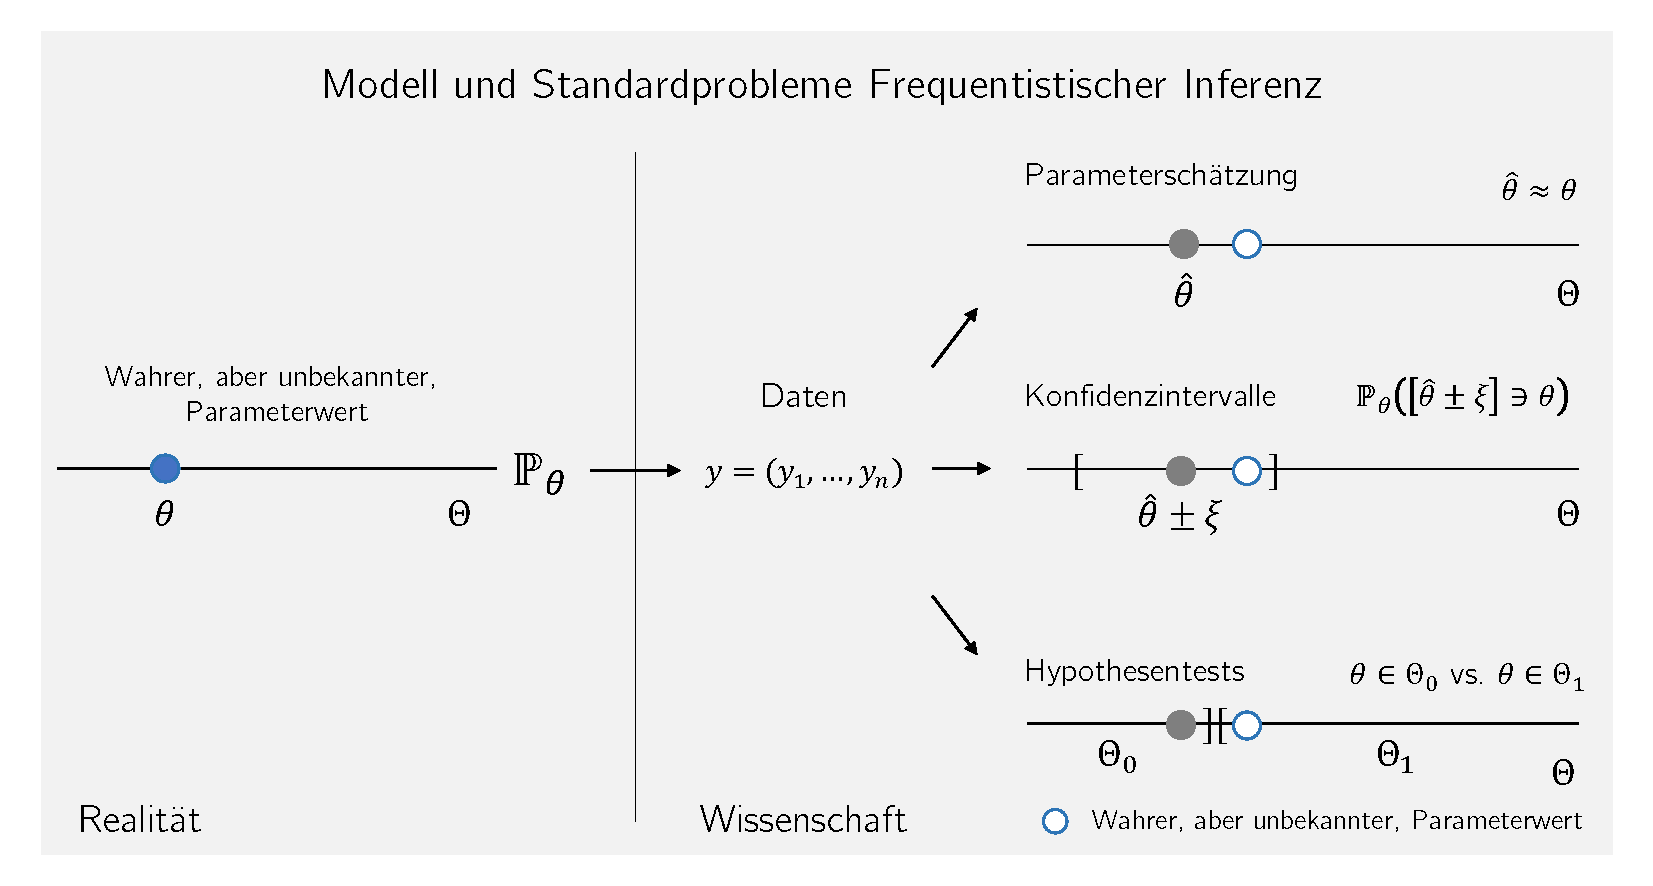
\includegraphics[width=1\linewidth]{10_Abbildungen/wtfi_10_frequentistische_inferenz} \end{center}
\end{frame}

\begin{frame}{}
\protect\hypertarget{section-3}{}
\begin{center}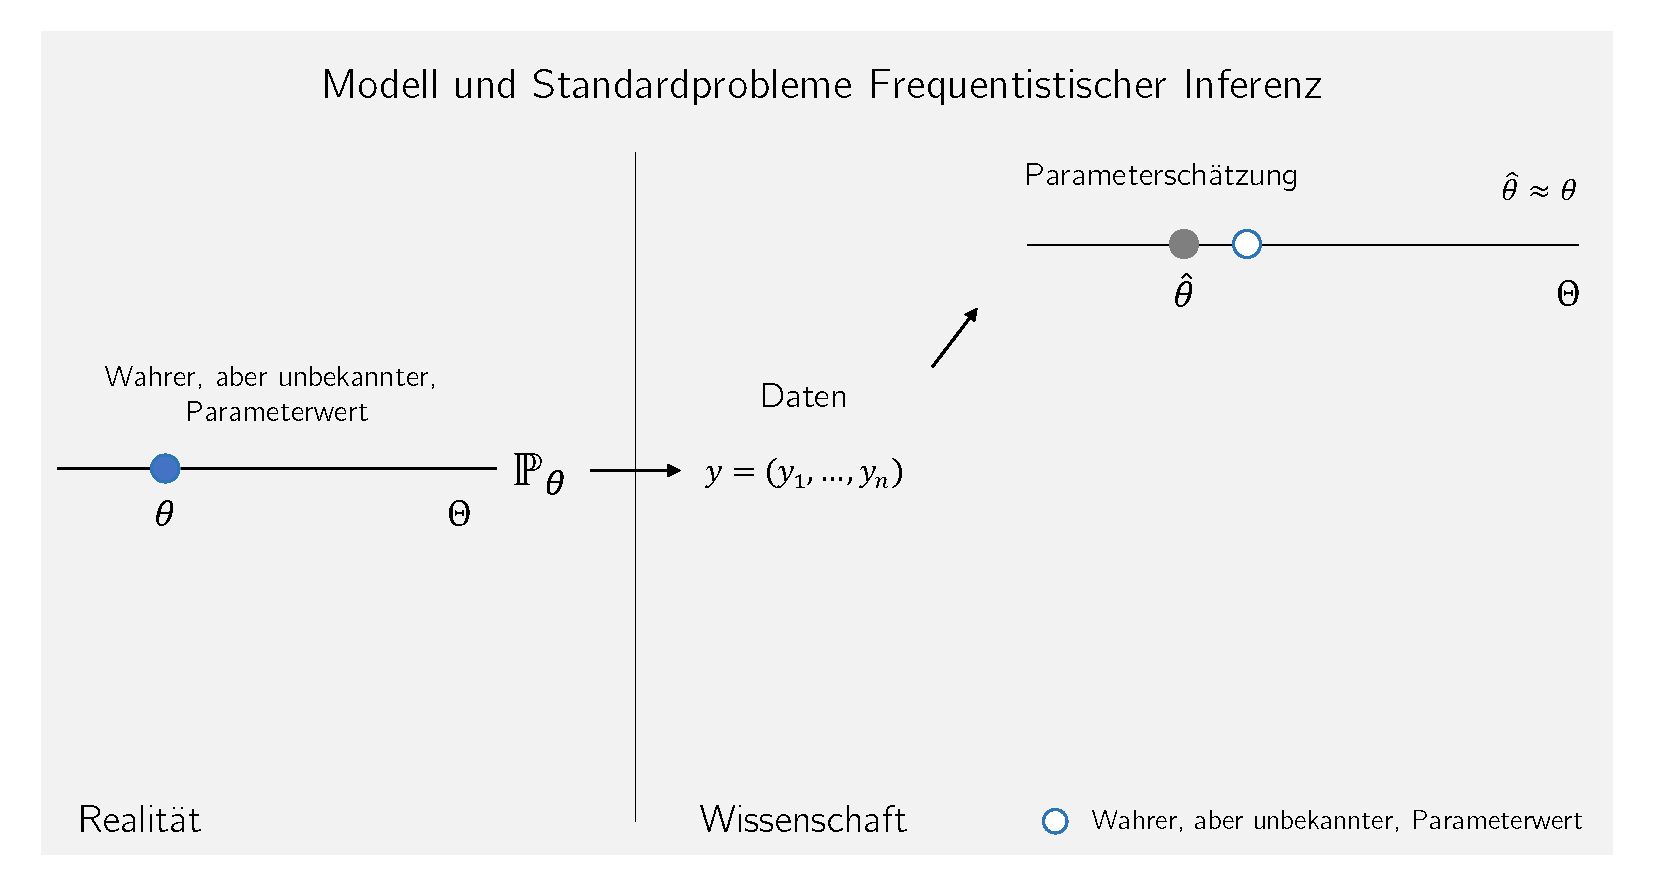
\includegraphics[width=1\linewidth]{10_Abbildungen/wtfi_10_frequentistische_inferenz_parameterschätzung} \end{center}
\end{frame}

\begin{frame}{}
\protect\hypertarget{section-4}{}
Standardannahmen Frequentistischer Inferenz

\footnotesize

\(\mathcal{M}\) sei ein statistisches Modell mit Stichprobe
\(\ups_1,...,\ups_n \sim p_\theta\). \textbf{Es wird angenommen, dass
ein konkret vorliegender Datensatz
\(y = (y_1,...,y_n) \in \mathbb{R}^n\) eine der möglichen Realisierungen
von \(\ups_1,...,\ups_n \sim p_\theta\) ist.} Aus Frequentistischer
Sicht kann man eine Studie unter gleichen Umständen unendlich oft
wiederholen und zu jedem Datensatz Schätzer oder Statistiken auswerten,
z.B. das Stichprobenmittel:

\footnotesize
\begin{itemize}
\item[] Datensatz (1) : $y^{(1)} = \left(y_1^{(1)}, y_2^{(1)}, ...,y_n^{(1)}\right)$
                        mit $\bar{y}_n^{(1)} = \frac{1}{n}\sum_{i=1}^n y_i^{(1)}$
\item[] Datensatz (2) : $y^{(2)} = \left(y_1^{(2)}, y_2^{(2)}, ...,y_n^{(2)}\right)$
                        mit $\bar{y}_n^{(2)} = \frac{1}{n}\sum_{i=1}^n y_i^{(2)}$
\item[] Datensatz (3) : $y^{(3)} = \left(y_1^{(3)}, y_2^{(3)}, ...,y_n^{(3)}\right)$
                        mit $\bar{y}_n^{(3)} = \frac{1}{n}\sum_{i=1}^n y_i^{(3)}$
\item[] Datensatz (4) : $y^{(4)} = \left(y_1^{(4)}, y_2^{(4)}, ...,y_n^{(4)}\right)$
                        mit $\bar{y}_n^{(4)} = \frac{1}{n}\sum_{i=1}^n y_i^{(4)}$
\item[] Datensatz (5) : $y^{(5)} = ...$
\end{itemize}

Um die Qualität statistischer Methoden zu beurteilen betrachtet die
Frequentistische Statistik deshalb die Wahrscheinlichkeitsverteilungen
von Schätzern und Statistiken unter Annahme von
\(\ups_1,...,\ups_n \sim p_\theta\). Was zum Beispiel ist die Verteilung
der \(\bar{y}_n^{(1)}\), \(\bar{y}_n^{(2)}\), \(\bar{y}_n^{(3)}\),
\(\bar{y}_n^{(4)}\), \ldots{} also die Verteilung der Zufallsvariable
\(\bar{\ups}_n\)?

Wenn eine statistische Methode im Sinne der Frequentistischen
Standardannahmen ``gut'' ist, dann heißt das also, dass sie bei häufiger
Anwendung ``im Mittel gut'' ist. Im Einzelfall, also im Normalfall nur
eines vorliegenden Datensatzes, kann sie auch ``schlecht'' sein.
\end{frame}

\begin{frame}{}
\protect\hypertarget{section-5}{}
\large
\vfill
\setstretch{2.3}

Grundbegriffe

Maximum-Likelihood Schätzer

Schätzereigenschaften bei endlichen Stichproben

Asymptotische Schätzereigenschaften

Eigenschaften von Maximum-Likelihood Schätzern

Selbstkontrollfragen \vfill
\end{frame}

\begin{frame}{}
\protect\hypertarget{section-6}{}
\large
\vfill
\setstretch{2.3}

\textbf{Grundbegriffe}

Maximum-Likelihood Schätzer

Schätzereigenschaften bei endlichen Stichproben

Asymptotische Schätzereigenschaften

Eigenschaften von Maximum-Likelihood Schätzern

Selbstkontrollfragen \vfill
\end{frame}

\begin{frame}{Grundbegriffe}
\protect\hypertarget{grundbegriffe}{}
\small
\begin{definition}[Parameterpunktschätzer]
\justifying
$\mathcal{M} := (\mathcal{Y}, \mathcal{A}, \{\mathbb{P}_\theta|\theta \in \Theta\})$
sei ein statistisches Modell, $(\Theta,\mathcal{S})$ sei ein Messraum und
$\hat{\theta} : \mathcal{Y} \to \Theta$ sei eine Abbildung. Dann nennen wir
$\hat{\theta}$ einen \textit{Parameterpunktschätzer} für $\theta$.
\end{definition}

Bemerkungen

\begin{itemize}
\tightlist
\item
  Parameterpunktschätzer nennt man auch einfach
  \emph{Parameterschätzer}.
\item
  Parameterpunktschätzer sind Schätzer mit \(\tau := \mbox{id}_\Theta\)
\item
  Parameterschätzer nehmen Zahlwerte in \(\Theta\) an.
\item
  Notationstechnisch wird oft nicht zwischen \(\hat{\theta}\) und
  \(\hat{\theta}(y)\) unterschieden.
\end{itemize}
\end{frame}

\begin{frame}{Grundbegriffe}
\protect\hypertarget{grundbegriffe-1}{}
\justifying

Prinzipien zur Gewinnung von Parameterschätzern

\small

Die Definition eines Parameterschätzers macht keine Aussage darüber, wie
man Parameterschätzer findet. Zur Gewinnung von Parameterschätzern in
statistischen Modellen haben sich deshalb verschiedene Prinzipien
etabliert. Populäre Prinzipien zur Gewinnung von Parameterschätzern sind

\begin{itemize}
\tightlist
\item
  Momentenmethode (\(\approx\) est. 1890)
\item
  Maximum-Likelihood Methode (\(\approx\) est. 1920)
\item
  M-, Z-, W-Schätzung (\(\approx\) est. 1960)
\end{itemize}

\emph{Perse} garantiert keine der obengenannten Methoden, dass die mit
ihrer Hilfe generierten Parameterschätzer in einem wohldefinierten Sinn
gute Schätzer sind.

Die Eigenschaften von durch die Maximum-Likelihood Methode generierten
Schätzern sind generell wünschenswert. Wir betrachten also in der Folge
nur die Maximum-Likelihood Methode genauer. Mithilfe der
Maximum-Likelihood Methode generierte Parameterpunktschätzer nennen wir
\emph{Maximum-Likelihood (ML) Schätzer}.
\end{frame}

\begin{frame}{}
\protect\hypertarget{section-7}{}
\large
\vfill
\setstretch{2.3}

Grundbegriffe

\textbf{Maximum-Likelihood Schätzer}

Schätzereigenschaften bei endlichen Stichproben

Asymptotische Schätzereigenschaften

Eigenschaften von Maximum-Likelihood Schätzern

Selbstkontrollfragen \vfill
\end{frame}

\begin{frame}{Maximum-Likelihood Schätzer}
\protect\hypertarget{maximum-likelihood-schuxe4tzer}{}
\small
\begin{definition}[Likelihood-Funktion und Log-Likelihood-Funktion]
\justifying
$\mathcal{M}$ sei ein parametrisches statistisches Produktmodell mit WMF oder WDF $p_\theta$,
also $\ups_1,...,\ups_n \sim p_\theta$. Dann ist die \textit{Likelihood Funktion} definiert als
\begin{equation}
L_n : \Theta \to [0,\infty[, \theta \mapsto L_n(\theta) := \prod_{i=1}^n p_\theta(y_i)
\end{equation}
und die \textit{Log-Likelihood-Funktion} ist definiert als
\begin{equation}
\mathcal{\ell}_n : \Theta \to \mathbb{R}, \theta \mapsto \ell_n(\theta) := \ln L_n(\theta).
\end{equation}
\end{definition}

\footnotesize

Bemerkungen

\begin{itemize}
\tightlist
\item
  \(L_n\) ist eine Funktion des Parameters eines statistischen Modells.
\item
  Werte von \(L_n\) sind die gemeinsamen Wahrscheinlichkeitsmassen bzw.
  -dichten von Datenwerten \(y_1,...,y_n\).
\item
  Generell gibt es keinen Grund anzunehmen, dass \(L_n\) über \(\Theta\)
  zu 1 integriert.
\item
  Die Likelihood-Funktion ist also keine WMF oder WDF.
\item
  Die Log-Likelihood-Funktion ist die logarithmierte
  Likelihood-Funktion.
\end{itemize}
\end{frame}

\begin{frame}{Maximum-Likelihood Schätzer}
\protect\hypertarget{maximum-likelihood-schuxe4tzer-1}{}
\small
\begin{definition}[Maximum-Likelihood Schätzer]
\justifying
$\mathcal{M}$ sei ein parametrisches statistisches Produktmodell mit Parameter
$\theta \in \Theta$. Ein \textit{Maximum-Likelihood Schätzer} von $\theta$
ist definiert als
\begin{equation}
\hat{\theta}^{\mbox{\tiny ML}}_n : \mathcal{Y} \to \Theta,
y \mapsto \hat{\theta}^{\mbox{\tiny ML}}_n(y)
:= \argmax_{\theta \in \Theta} L_n(\theta)
=  \argmax_{\theta \in \Theta} \ell_n(\theta).
\end{equation}
\end{definition}

\footnotesize

Bemerkungen

\begin{itemize}
\tightlist
\item
  \justifying \(L_n(\theta) := \prod_{i=1}^n p_\theta(y_i)\) hängt von
  \(y := (y_1,...,y_n)\) ab, also hängt auch
  \(\hat{\theta}^{\mbox{\tiny ML}}_n(y)\) von \(y\) ab.
\item
  Weil \(\ln\) monoton steigend ist, entspricht eine Maximumstelle von
  \(\ell_n\) einer Maximumstelle von \(L_n\).
\item
  Das Arbeiten mit der Log-Likelihood-Funktion ist oft einfacher als mit
  der Likelihood Funktion.
\item
  Multiplikation von \(L_n\) mit einer positiven Konstante, die nicht
  von \(\theta\) abhängt, verändert einen Maximum-Likelihood Schätzer
  nicht, konstante additive Terme in der Log-Likelihood können also
  vernachlässigt werden.
\item
  Maximum-Likelihood Schätzung ist ein Optimierungsproblem
\end{itemize}
\end{frame}

\begin{frame}{Maximum-Likelihood Schätzer}
\protect\hypertarget{maximum-likelihood-schuxe4tzer-2}{}
\setstretch{1.8}

Vorgehen zur Gewinnung von Maximum-Likelihood Schätzern

\begin{enumerate}
[(1)]
\tightlist
\item
  Formulierung der Log-Likelihood-Funktion.
\item
  Auswertung der Ableitung der Log-Likelihood-Funktion und Nullsetzen.
\item
  Auflösen nach potentiellen Maximumstellen.
\end{enumerate}

Dabei nutzt man typischerweise

\begin{itemize}
\tightlist
\item
  Methoden der analytischen Optimierung in klassischen Beispielen\\
\item
  Methoden der numerischen Optimierung im Anwendungskontext.
\end{itemize}
\end{frame}

\begin{frame}{Maximum-Likelihood Schätzer}
\protect\hypertarget{maximum-likelihood-schuxe4tzer-3}{}
Beispiel (Bernoullimodell)

\small

\(\mathcal{M}\) sei das Bernoullimodell, also
\(\ups_1,...,\ups_n \sim \mbox{Bern}(\mu)\).

\noindent (1) Formulierung der Log-Likelihood-Funktion

\footnotesize

Es gilt \begin{equation}
L_n : ]0,1[ \to ]0,1[,
\mu \mapsto L_n(\mu)
:= \prod_{i=1}^n \mu^{y_i}(1 - \mu)^{1-y_i}
 = \mu^{\sum_{i=1}^n y_i}(1 - \mu)^{n - \sum_{i=1}^n y_i}.
\end{equation} Logarithmieren ergibt \begin{equation}
\ell_n : ]0,1[ \to \mathbb{R}, \mu \mapsto  \ell_n(\mu)
= \ln \mu \sum_{i=1}^n y_i + \ln (1- \mu) \left(n - \sum_{i=1}^n y_i \right).
\end{equation}
\end{frame}

\begin{frame}{Maximum-Likelihood Schätzer}
\protect\hypertarget{maximum-likelihood-schuxe4tzer-4}{}
Beispiel (Bernoullimodell)

\small

\noindent (2) Auswertung der Ableitung der Log-Likelihood-Funktion und
Nullsetzen

\footnotesize

Es gilt \begin{align}
\begin{split}
\frac{d}{d\mu} \ell_n(\mu)
& = \frac{d}{d\mu}\left(\ln \mu \sum_{i=1}^n y_i + \ln (1- \mu) \left(n - \sum_{i=1}^n y_i \right)\right)  \\
& = \frac{d}{d\mu} \ln \mu \sum_{i=1}^n y_i  + \frac{d}{d\mu} \ln (1 - \mu) \left(n - \sum_{i=1}^n y_i \right)  \\
& = \frac{1}{\mu}\sum_{i=1}^n y_i  -  \frac{1}{1-\mu} \left(n - \sum_{i=1}^n y_i \right).
\end{split}
\end{align} Die sogenannte \textit{Maximum-Likelihood Gleichung} ergibt
sich in diesem Beispiel also zu \begin{equation}
\frac{1}{\hat{\mu}_{n}^{\mbox{\tiny ML}}}\sum_{i=1}^n y_i - \frac{1}{1-\hat{\mu}_{n}^{\mbox{\tiny ML}}} \left(n - \sum_{i=1}^n y_i \right) = 0.
\end{equation}
\end{frame}

\begin{frame}{Maximum-Likelihood Schätzer}
\protect\hypertarget{maximum-likelihood-schuxe4tzer-5}{}
Beispiel (Bernoullimodell)

\small

\noindent (3) Auflösen nach potentiellen Maximumstellen

\footnotesize

Es gilt \begin{align}
\begin{split}
\frac{1}{\hat{\mu}_{n}^{\mbox{\tiny ML}}}\sum_{i=1}^n y_i - \frac{1}{1-\hat{\mu}_{n}^{\mbox{\tiny ML}}} \left(n - \sum_{i=1}^n y_i \right) & = 0 \\
\Leftrightarrow
\hat{\mu}_{n}^{\mbox{\tiny ML}}(1 - \hat{\mu}_{n}^{\mbox{\tiny ML}})\left(\frac{1}{\hat{\mu}_{n}^{\mbox{\tiny ML}}}\sum_{i=1}^n y_i - \frac{1}{1-\hat{\mu}_{n}^{\mbox{\tiny ML}}} \left(n - \sum_{i=1}^n y_i \right) \right) & = 0 \\
\Leftrightarrow
\sum_{i=1}^n y_i - \hat{\mu}_{n}^{\mbox{\tiny ML}} \sum_{i=1}^n y_i - n \hat{\mu}_{n}^{\mbox{\tiny ML}}  + \hat{\mu}_{n}^{\mbox{\tiny ML}}\sum_{i=1}^n y_i & = 0 \\
\Leftrightarrow
n \hat{\mu}_{n}^{\mbox{\tiny ML}}  & = \sum_{i=1}^n y_i \\
\Leftrightarrow
\hat{\mu}_{n}^{\mbox{\tiny ML}}  & = \frac{1}{n} \sum_{i=1}^n y_i. \\
\end{split}
\end{align}
\end{frame}

\begin{frame}{Maximum-Likelihood Schätzer}
\protect\hypertarget{maximum-likelihood-schuxe4tzer-6}{}
Beispiel (Bernoullimodell) \vspace{2mm}

\small

\(\hat{\mu}_{n}^{\mbox{\tiny ML}} = \frac{1}{n}\sum_{i=1}^n y_i\) ist
also ein potentieller Maximum-Likelihood Schätzer von \(\mu\). Dies kann
durch Betrachten der zweiten Ableitung von \(\ell_n\) verifiziert
werden, worauf hier verzichtet werden soll. \begin{equation}
\hat{\mu}_{n}^{\mbox{\tiny ML}} : \{0,1\}^n \to [0,1],
y \mapsto \hat{\mu}_{n}^{\mbox{\tiny ML}}(y):= \frac{1}{n}\sum_{i=1}^n y_i
\end{equation} ist also ein Maximum-Likelihood Schätzer von \(\mu\) im
Bernoullimodell.
\end{frame}

\begin{frame}{Maximum-Likelihood Schätzer}
\protect\hypertarget{maximum-likelihood-schuxe4tzer-7}{}
Beispiel (Normalverteilungsmodell)

\small

\(\mathcal{M}\) sei das Normalverteilungsmodell, also
\(\ups_1,...,\ups_n \sim N\left(\mu,\sigma^2\right)\)

\noindent (1) Formulierung der Log-Likelihood-Funktion

\footnotesize

Es gilt \begin{align}
\begin{split}
L_n : \mathbb{R} \times \mathbb{R}_{>0} \to \mathbb{R}_{>0},
(\mu,\sigma^2) \mapsto L_n(\mu,\sigma^2)
:= & \prod_{i=1}^n \frac{1}{\sqrt{2\pi \sigma^2}}\exp\left(-\frac{1}{2\sigma^2}(y_i-\mu)^2\right) \\
 = & \left(2 \pi \sigma^2\right)^{-\frac{n}{2}}\exp\left(-\frac{1}{2\sigma^2}\sum_{i=1}^n(y_i-\mu)^2\right). \\
\end{split}
\end{align} Logarithmieren ergibt \begin{equation}
\ell_n : \mathbb{R} \times \mathbb{R}_{>0} \to \mathbb{R},
(\mu,\sigma^2) \mapsto \mathcal{\ell}_n(\mu,\sigma^2)
= -\frac{n}{2} \ln 2\pi - \frac{n}{2} \ln \sigma^2  -\frac{1}{2\sigma^2}\sum_{i=1}^n(y_i-\mu)^2.
\end{equation}
\end{frame}

\begin{frame}{Maximum-Likelihood Schätzer}
\protect\hypertarget{maximum-likelihood-schuxe4tzer-8}{}
Beispiel (Normalverteilungsmodell)

\small

\noindent (2) Auswertung der Ableitung der Log-Likelihood-Funktion und
Nullsetzen

\footnotesize

Es ergibt sich \begin{equation}
\frac{d}{d\mu} \ell_n(\mu)
 = - \frac{d}{d\mu} \frac{1}{2\sigma^2}\sum_{i=1}^n(y_i-\mu)^2
 = - \frac{1}{2\sigma^2}\sum_{i=1}^n \frac{d}{d\mu} (y_i-\mu)^2
 = \frac{1}{\sigma^2}\sum_{i=1}^n (y_i-\mu).
\end{equation} Weiterhin ergibt sich \begin{align}
\begin{split}
\frac{d}{d\sigma^2} \ell_n(\sigma^2)
= - \frac{n}{2} \frac{d}{d\sigma^2} \ln \sigma^2  - \frac{d}{d\sigma^2} \frac{1}{2\sigma^2}\sum_{i=1}^n(y_i-\mu)^2
= - \frac{n}{2 \sigma^2} + \frac{1}{2\sigma^4}\sum_{i=1}^n(y_i-\mu)^2.
\end{split}
\end{align} Die Maximum-Likelihood Gleichungen haben also die Form
\begin{align}
\begin{split}
\sum_{i=1}^n (y_i-\hat{\mu}_{n}^{\mbox{\tiny ML}}) & = 0 \\
- \frac{n}{2 \hat{\sigma}^{2^{\mbox{\tiny ML}}}_n} + \frac{1}{2\hat{\sigma}^{4^{\mbox{\tiny ML}}}_n}\sum_{i=1}^n(y_i-\mu)^2 & = 0
\end{split}
\end{align}
\end{frame}

\begin{frame}{Maximum-Likelihood Schätzer}
\protect\hypertarget{maximum-likelihood-schuxe4tzer-9}{}
Beispiel (Normalverteilungsmodell)

\small

\noindent (3) Auflösen nach potentiellen Maximumstellen

\footnotesize

Es ergibt sich \begin{equation}
\sum_{i=1}^n (y_i-\hat{\mu}_{n}^{\mbox{\tiny ML}})  = 0
\Leftrightarrow \sum_{i=1}^n y_i  = n\hat{\mu}_{n}^{\mbox{\tiny ML}}
\Leftrightarrow \hat{\mu}_{n}^{\mbox{\tiny ML}} = \frac{1}{n}\sum_{i=1}^n y_i.
\end{equation} Also ist
\(\hat{\mu}_{n}^{\mbox{\tiny ML}} = n^{-1}\sum_{i=1}^n y_i\) ein
potentieller Maximum-Likelihood Schätzer von \(\mu\). Einsetzen ergibt
dann\\
\begin{align}
\begin{split}
- \frac{n}{2 \hat{\sigma}^{2^{\mbox{\tiny ML}}}_n} + \frac{1}{2\hat{\sigma}^{4^{\mbox{\tiny ML}}}_n}\sum_{i=1}^n(y_i-\hat{\mu}_{n}^{\mbox{\tiny ML}})^2 & = 0 \\
\Leftrightarrow
- n\hat{\sigma}^{2^{\mbox{\tiny ML}}}_n + \sum_{i=1}^n(y_i-\hat{\mu}_{n}^{\mbox{\tiny ML}})^2 & = 0 \\
\Leftrightarrow
\hat{\sigma}^{2^{\mbox{\tiny ML}}}_n & = \frac{1}{n} \sum_{i=1}^n(y_i-\hat{\mu}_{n}^{\mbox{\tiny ML}})^2.
\end{split}
\end{align}
\(\hat{\sigma}^{2^{\mbox{\tiny ML}}}_n = n^{-1}\sum_{i=1}^n(y_i-\hat{\mu}_{n}^{\mbox{\tiny ML}})^2\)
ist also ein potentieller Maximum-Likelihood Schätzer von \(\sigma^2\).
\end{frame}

\begin{frame}{Maximum-Likelihood Schätzer}
\protect\hypertarget{maximum-likelihood-schuxe4tzer-10}{}
Beispiel (Normalverteilungsmodell)

\vspace{2mm}

\small

Beide potentiellen Maximum-Likelihood Schätzer können durch Betrachten
der zweiten Ableitung von \(\ell_n\) verifiziert werden, worauf hier
verzichtet werden soll.

Also sind \begin{equation}
\hat{\mu}_{n}^{\mbox{\tiny ML}} :
\mathbb{R}^n \to \mathbb{R}, y \mapsto \hat{\mu}_{n}^{\mbox{\tiny ML}}(y)
:= \frac{1}{n}\sum_{i=1}^n y_i
\end{equation} und \begin{equation}
\hat{\sigma}_n^{2^{\mbox{\tiny ML}}} :
\mathbb{R}^n \to \mathbb{R}_{\ge 0},
y \mapsto \hat{\sigma}_n^{2^{\mbox{\tiny ML}}}(y)
:= \frac{1}{n}\sum_{i=1}^n \left(y_i - \hat{\mu}_{n}^{\mbox{\tiny ML}}\right)^2.
\end{equation} die Maximum-Likelihood Schätzer von \(\mu\) und
\(\sigma^2\) im Normalverteilungsmodell.
\(\hat{\mu}_{n}^{\mbox{\tiny ML}}\) ist identisch mit dem
Stichprobenmittel \(\bar{\ups}_n\),
\(\hat{\sigma}_{n}^{2^{\mbox{\tiny ML}}}\) ist dagegen nicht identisch
mit der Stichprobenvarianz \(S^2_n\).
\end{frame}

\begin{frame}[t]{Maximum-Likelihood Schätzer}
\protect\hypertarget{maximum-likelihood-schuxe4tzer-11}{}
Beispiel \textbar{} Evidenzbasierte Evaluation von Psychotherapie bei
Depression

\begin{center}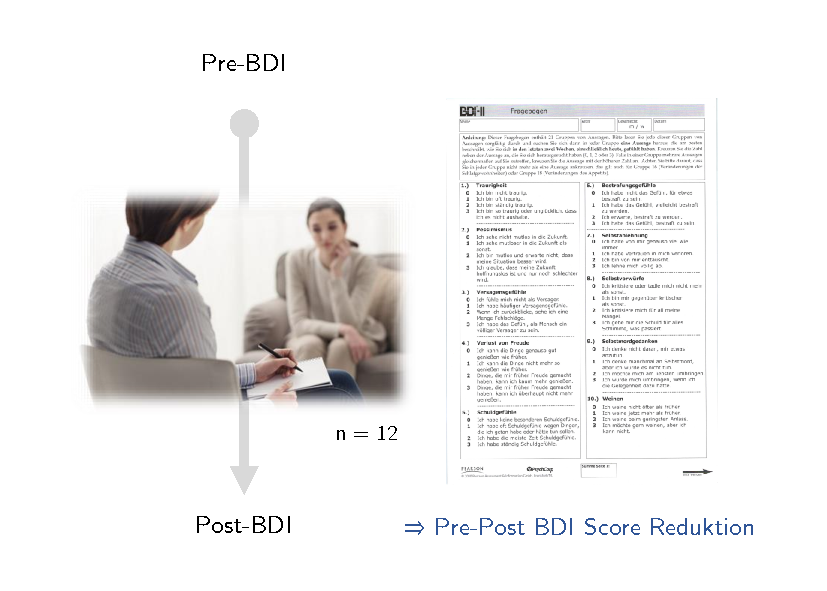
\includegraphics[width=0.9\linewidth]{10_Abbildungen/wtfi_10_messplan} \end{center}
\end{frame}

\begin{frame}[fragile,t]{Maximum-Likelihood Schätzer}
\protect\hypertarget{maximum-likelihood-schuxe4tzer-12}{}
Beispiel \textbar{} Evidenzbasierte Evaluation von Psychotherapie bei
Depression

\small
\vspace{2mm}

\footnotesize

\begin{Shaded}
\begin{Highlighting}[]
\NormalTok{fname }\OtherTok{=} \FunctionTok{file.path}\NormalTok{(}\FunctionTok{getwd}\NormalTok{(), }\StringTok{"10\_Parameterschätzung.csv"}\NormalTok{)}
\NormalTok{D     }\OtherTok{=} \FunctionTok{read.table}\NormalTok{(fname, }\AttributeTok{sep =} \StringTok{","}\NormalTok{, }\AttributeTok{header =}\NormalTok{ T)}
\end{Highlighting}
\end{Shaded}

\vspace{2mm}

\begin{longtable}[]{@{}rr@{}}
\toprule()
i & BDI.Reduktion \\
\midrule()
\endhead
1 & -1 \\
2 & 3 \\
3 & -2 \\
4 & 9 \\
5 & 3 \\
6 & -2 \\
7 & 4 \\
8 & 5 \\
9 & 5 \\
10 & 1 \\
11 & 9 \\
12 & 4 \\
\bottomrule()
\end{longtable}
\end{frame}

\begin{frame}[t]{Maximum-Likelihood Schätzer}
\protect\hypertarget{maximum-likelihood-schuxe4tzer-13}{}
Beispiel \textbar{} Evidenzbasierte Evaluation von Psychotherapie bei
Depression \vspace{2mm}

\small

Für die Pre-Post BDI Score Reduktion \(\ups_i\) der \(i\)ten von \(n\)
Patient:innen legen wir das Modell \begin{equation}
\ups_{i} = \mu + \varepsilon_{i} \mbox{ mit } \varepsilon_{i} \sim N(0,\sigma^2) \mbox{ u.i.v. für } i = 1,...,n
\end{equation} zugrunde. Dabei wird die Pre-Post BDI Reduktion
\(\ups_i\) der \(i\)ten Patient:in also mithilfe einer über die Gruppe
von Patient:innen identischen Pre-Post BDI Score Reduktion
\(\mu \in \mathbb{R}\) und einer Patient:innen-spezifischen
normalverteilten Pre-Post BDI Score Reduktionsabweichung
\(\varepsilon_{i}\) erklärt

Wie gezeigt ist dieses Modell äquivalent zum Normalverteilungsmodell
\begin{equation}
\ups_1,...,\ups_n \sim N(\mu,\sigma^2).
\end{equation}

Die Standardprobleme der Frequentistischen Inferenz führen in diesem
Szenario auf folgende Fragen:

\begin{enumerate}
[(1)]
\tightlist
\item
  Was sind sinnvolle Tipps für die wahren, aber unbekannten,
  Parameterwerte \(\mu\) und \(\sigma^2\)?
\item
  Wie hoch ist im frequentistischen Sinn die mit diesen Tipps
  assoziierte Unsicherheit?
\item
  Entscheiden wir uns sinnvollerweise für die Hypothese, dass gilt
  \(\mu\neq 0\) ?
\end{enumerate}
\end{frame}

\begin{frame}[fragile,t]{Maximum-Likelihood Schätzer}
\protect\hypertarget{maximum-likelihood-schuxe4tzer-14}{}
Beispiel \textbar{} Evidenzbasierte Evaluation von Psychotherapie bei
Depression \vspace{2mm} \footnotesize

\begin{Shaded}
\begin{Highlighting}[]
\CommentTok{\# Einlesen und Auswahl der Daten}
\NormalTok{fname }\OtherTok{=} \FunctionTok{file.path}\NormalTok{(}\FunctionTok{getwd}\NormalTok{(), }\StringTok{"10\_Parameterschätzung.csv"}\NormalTok{)}
\NormalTok{D     }\OtherTok{=} \FunctionTok{read.table}\NormalTok{(fname, }\AttributeTok{sep =} \StringTok{","}\NormalTok{, }\AttributeTok{header =}\NormalTok{ T)}
\NormalTok{y     }\OtherTok{=}\NormalTok{ D}\SpecialCharTok{$}\NormalTok{BDI.Reduktion}

\CommentTok{\# ML Schätzung des Erwartungswertparameters}
\NormalTok{mu\_hat   }\OtherTok{=} \FunctionTok{mean}\NormalTok{(y)                           }\CommentTok{\# mean(y) berechnet das Stichprobenmittel}
\FunctionTok{print}\NormalTok{(mu\_hat)                                }\CommentTok{\# Ausgabe}
\end{Highlighting}
\end{Shaded}

\begin{verbatim}
> [1] 3.17
\end{verbatim}

\vspace{2mm}

\begin{Shaded}
\begin{Highlighting}[]
\CommentTok{\# ML Schätzung des Varianzparameters}
\NormalTok{n           }\OtherTok{=} \FunctionTok{length}\NormalTok{(y)                      }\CommentTok{\# Anzahl der Datenpunkte}
\NormalTok{sigsqr\_hat  }\OtherTok{=}\NormalTok{ ((n}\DecValTok{{-}1}\NormalTok{)}\SpecialCharTok{/}\NormalTok{n)}\SpecialCharTok{*}\FunctionTok{var}\NormalTok{(y)               }\CommentTok{\# var(y) berechnet die Stichprobenvarianz}
\FunctionTok{print}\NormalTok{(sigsqr\_hat)                            }\CommentTok{\# Ausgabe}
\end{Highlighting}
\end{Shaded}

\begin{verbatim}
> [1] 12.6
\end{verbatim}

\footnotesize

Basierend auf dem Prinzip der Maximum-Likelihood Schätzung sind also
\begin{equation}
\hat{\mu}_{12}^{\mbox{\tiny ML}} = 3.17,
\mbox{ und }
\hat{\sigma}^{2^{\mbox{\tiny ML}}}_{12} = 12.6
\end{equation} sinnvolle Tipps für \(\mu\) und \(\sigma^2\) basierend
auf den vorliegenden 12 Datenpunkten.
\end{frame}

\begin{frame}{}
\protect\hypertarget{section-8}{}
\large
\vfill
\setstretch{2.3}

Grundbegriffe

Maximum-Likelihood Schätzer

\textbf{Schätzereigenschaften bei endlichen Stichproben}

Asymptotische Schätzereigenschaften

Eigenschaften von Maximum-Likelihood Schätzern

Selbstkontrollfragen \vfill
\end{frame}

\begin{frame}{}
\protect\hypertarget{section-9}{}
Vorbemerkungen zu Frequentistischen Schätzereigenschaften

\footnotesize

Wir gehen von einem statistischem parametrischem Produktmodell
\(\mathcal{M} := \{\mathcal{Y},\mathcal{A}, \{\mathbb{P}_\theta| \theta \in \Theta\}\}\)
mit \(n\)-dimensionalen Stichprobenraum (z.B.
\(\mathcal{Y} := \mathbb{R}^n\)), \(d\)-dimensionalen Parameteraum
\(\Theta \subset \mathbb{R}^d\) und gegebener WMF oder WDF \(p_\theta\)
für alle \(\theta \in \Theta\) aus.
\(\ups := \ups_1,...,\ups_n \sim p_\theta\) bezeichnet die zu
\(\mathcal{M}\) gehörende Stichprobe unabhängig und identisch verteilter
Zufallsvariablen, es gilt also \(\ups_1 \sim p_\theta\) und
\(\ups_i \sim p_\theta\) für alle \(i = 1,...,n\).

Für einen Messraum \((\Sigma,S)\) sei
\(\hat{\tau} : \mathcal{Y} \to \Sigma\) ein Schätzer von
\(\tau : \Theta \to \Sigma\). Wir betrachten Erwartungswerts- Varianz-,
und Standardabweichungsschätzer, also Schätzer für \begin{align}
\begin{split}
\tau : \Theta \to \Sigma,\,
\theta \mapsto \tau(\theta)
\mbox{ mit }
\tau(\theta) := \mathbb{E}_\theta(\ups_1),
\tau(\theta) := \mathbb{V}_\theta(\ups_1), \mbox{ und }
\tau(\theta) := \mathbb{S}_\theta(\ups_1)
\end{split}
\end{align} respektive, sowie Parameterschätzer, also Schätzer für
\begin{equation}
\tau: \Theta \to \Sigma, \tau(\theta) := \theta.
\end{equation} In der Folge führen wir \emph{Frequentistische
Schätzereigenschaften} ein. Frequentistische Schätzereigenschaften
betrachten die Verteilung der Schätzwerte \(\hat{\tau}(y_1,...,y_n)\) in
Abhängigkeit von der Verteilung der Datennwerte
\(\ups := \ups_1,...,\ups_n\). Weil die Stichprobenwerte zufällig sind,
sind auch die Schätzwerte zufällig; ein Schätzer \(\hat{\tau}\) ist also
wie oben gesehen eine Zufallsvariable. Wir unterscheiden zwischen
\emph{Schätzereigenschaften bei endlichen Stichproben}, d.h.
Eigenschaften von \(\hat{\tau}_n\) für ein fixes \(n \in \mathbb{N}\)
(z.B. \(n = 12\)) und \emph{Asymptotischen Schätzereigenschaften}, d.h.
Eigenschaften von \(\hat{\tau}_n\) für unendlich groß werdende
Stichproben mit \(n \to \infty\).
\end{frame}

\begin{frame}{Schätzereigenschaften bei endlichen Stichproben}
\protect\hypertarget{schuxe4tzereigenschaften-bei-endlichen-stichproben}{}
\justifying

Schätzereigenschaften bei endlichen Stichproben

\footnotesize

Wir betrachten vier Aspekte von Schätzereigenschaften bei endlichen
Stichproben.

\begin{enumerate}
[(1)]
\tightlist
\item
  Erwartungstreue
\item
  Varianz und Standardfehler
\item
  Mittlerer Quadratischer Fehler
\item
  Cramér-Rao Ungleichung
\end{enumerate}

Intuitiv haben diese folgende Bedeutungen:

\begin{enumerate}
[(1)]
\item
  \justifying Ein Schätzer \(\hat{\tau}_n\) heißt \emph{erwartungstreu},
  wenn sein Erwartungswert dem wahren, aber unbekannten, Wert
  \(\tau(\theta)\) für alle \(\theta \in \Theta\) gleicht.
\item
  Die \emph{Varianz} eines Schätzers \(\hat{\tau}_n\) ist die Varianz
  der Zufallsvariable \(\hat{\tau}_n(\ups)\). Der \emph{Standardfehler}
  eines Schätzers \(\hat{\tau}_n\) ist die Standardabweichung der
  Zufallsvariable \(\hat{\tau}_n(\ups)\).
\item
  Der \emph{mittlere quadratische Fehler} von \(\hat{\tau}_n\) ist der
  Erwartungswert der quadrierten Abweichung von \(\hat{\tau}_n(\ups)\)
  von \(\tau(\theta)\) über Stichproben vom Umfang \(n\).
\item
  Die \emph{Cramér-Rao-Ungleichung} gibt eine untere Schranke für die
  Varianz erwartungstreuer Schätzer an. Ein erwartungstreuer Schätzer
  mit Varianz gleich der in der Cramér-Rao-Ungleichung gegebenen unteren
  Schranke hat die kleinstmögliche Varianz aller erwartungstreuen
  Schätzer und ist in diesem Sinne ein optimaler Schätzer. Wir vertiefen
  die Cramér-Rao-Ungleichung lediglich in einem nicht klausurrelevanten
  Appendix.
\end{enumerate}
\end{frame}

\begin{frame}{\small Schätzereigenschaften bei endlichen Stichproben
\textbar{} Erwartungstreue}
\protect\hypertarget{schuxe4tzereigenschaften-bei-endlichen-stichproben-erwartungstreue}{}
\small
\begin{definition}[Fehler, Systematischer Fehler, und Erwartungstreue]
$\ups := \ups_1,...,\ups_n \sim  p_\theta$ sei eine Stichprobe und $\hat{\tau}_n$ sei ein Schätzer für $\tau$.
\begin{itemize}
\item Der \textit{Fehler} von $\hat{\tau}_n$ ist definiert als
\begin{equation}
\hat{\tau}_n(\ups) - \tau(\theta).
\end{equation}
\item Der \textit{systematische Fehler (Bias)} von $\hat{\tau}_n$ ist definiert als
\begin{equation}
\mbox{B}(\hat{\tau}_n) := \mathbb{E}_{\theta}(\hat{\tau}_n(\ups)) - \tau(\theta).
\end{equation}
\item $\hat{\tau}_n$ heißt \textit{erwartungstreu (unbiased)}, wenn
\begin{equation}
\mbox{B}(\hat{\tau}_n) = 0\Leftrightarrow
\mathbb{E}_{\theta}(\hat{\tau}_n(\ups)) = \tau(\theta) \mbox{ für alle } \theta \in \Theta, n \in \mathbb{N}.
\end{equation}
Andernfalls heißt $\hat{\tau}_n$  \textit{verzerrt (biased)}.
\end{itemize}
\end{definition}

\footnotesize

Bemerkungen

\begin{itemize}
\tightlist
\item
  Der Fehler hängt von einer Realisation der Stichprobe ab.
\item
  Der systematische Fehler ist der erwartete Fehler über viele
  Stichprobenrealisationen.
\item
  Ein Parameterschätzer ist erwartungstreu, wenn
  \(\mathbb{E}_{\theta}(\hat{\theta}_n(\ups)) = \theta\).
\end{itemize}
\end{frame}

\begin{frame}{\small Schätzereigenschaften bei endlichen Stichproben
\textbar{} Erwartungstreue}
\protect\hypertarget{schuxe4tzereigenschaften-bei-endlichen-stichproben-erwartungstreue-1}{}
\small
\begin{theorem}[Erwartungstreue von Stichprobenmittel und Stichprobenvarianz]
\justifying
\normalfont
$\ups_1,...,\ups_n \sim p_\theta$ sei die Stichprobe eines statistischen parametrischen Produktmodells $\mathcal{M}$.
\begin{itemize}
\item Das Stichprobenmittel
\begin{equation}
\bar{\ups}_n := \frac{1}{n}\sum_{i=1}^n \ups_i
\end{equation}
ist ein erwartungstreuer Schätzer des Erwartungswerts $\mathbb{E}_\theta(\ups_1)$.
\vspace{1mm}
\item Die Stichprobenvarianz
\begin{equation}
S^2_n := \frac{1}{n-1}\sum_{i=1}^n (\ups_i - \bar{\ups}_n)^2
\end{equation}
ist ein erwartungstreuer Schätzer der Varianz $\mathbb{V}_\theta(\ups_1)$.
\end{itemize}
\end{theorem}
\end{frame}

\begin{frame}{\small Schätzereigenschaften bei endlichen Stichproben
\textbar{} Erwartungstreue}
\protect\hypertarget{schuxe4tzereigenschaften-bei-endlichen-stichproben-erwartungstreue-2}{}
\footnotesize

\underline{Beweis}

Um die Notation zu vereinfachen, definieren wir
\(\mathbb{E} := \mathbb{E}_\theta\) und
\(\mathbb{V} := \mathbb{V}_\theta\). Mit der Linearität von
Erwartungswerten ergibt sich dann \begin{align*}
\mathbb{E}(\bar{\ups}_n)
= \mathbb{E} \left(\frac{1}{n}\sum_{i=1}^n  \ups_i \right)
= \frac{1}{n}\sum_{i=1}^n  \mathbb{E}\left( \ups_i \right)
= \frac{1}{n}\sum_{i=1}^n  \mathbb{E}\left( \ups_1 \right)
= \frac{1}{n} n  \mathbb{E}\left( \ups_1 \right)
=  \mathbb{E}\left( \ups_1 \right).
\end{align*} Dies zeigt die Erwartungstreue des Stichprobenmittels als
Schätzer des Erwartungswertes.

Um die Erwartungstreue der Stichprobenvarianz zu zeigen, halten wir
zunächst fest, dass \begin{equation*}
\mathbb{V}(\bar{\ups}_n)
= \mathbb{V}\left(\frac{1}{n} \sum_{i=1}^n \ups_i \right)
= \frac{1}{n^2} \sum_{i=1}^n \mathbb{V}\left( \ups_i \right)
= \frac{1}{n^2} \sum_{i=1}^n  \mathbb{V}\left( \ups_1 \right)
= \frac{1}{n^2} n \mathbb{V}\left( \ups_1 \right)
= \frac{\mathbb{V}\left( \ups_1 \right)}{n}.
\end{equation*} Weiterhin gilt, wie im Folgenden gezeigt, \begin{align*}
\sum_{i=1}^n \left(\ups_i - \bar{\ups}_n\right)^2 = \sum_{i=1}^n (\ups_i - \mu)^2 - n(\bar{\ups}_n - \mu)^2.
\end{align*}
\end{frame}

\begin{frame}{\small Schätzereigenschaften bei endlichen Stichproben
\textbar{} Erwartungstreue}
\protect\hypertarget{schuxe4tzereigenschaften-bei-endlichen-stichproben-erwartungstreue-3}{}
\vspace{-2mm}
\footnotesize

\begin{align}
\begin{split}
\sum_{i=1}^n \left(\ups_i - \bar{\ups}_n\right)^2
& = \sum_{i=1}^n \left(\ups_i - \mu - \bar{\ups}_n + \mu \right)^2 \\
& = \sum_{i=1}^n \left((\ups_i - \mu) - (\bar{\ups}_n - \mu) \right)^2 \\
& = \sum_{i=1}^n (\ups_i-\mu)^2 - 2(\bar{\ups}_n-\mu)\left(\sum_{i=1}^n(\ups_i-\mu)\right) + \sum_{i=1}^n (\bar{\ups}_n-\mu)^2 \\
& = \sum_{i=1}^n (\ups_i-\mu)^2 - 2(\bar{\ups}_n-\mu)\left(\sum_{i=1}^n\ups_i- n\mu\right) + n(\bar{\ups}_n-\mu)^2 \\
& = \sum_{i=1}^n (\ups_i-\mu)^2 - 2(\bar{\ups}_n-\mu)\left(n\left(\frac{1}{n}\sum_{i=1}^n\ups_i\right)- n\mu\right) + n(\bar{\ups}_n-\mu)^2 \\
& = \sum_{i=1}^n (\ups_i-\mu)^2 - 2n(\bar{\ups}_n-\mu)^2 + n(\bar{\ups}_n-\mu)^2 \\
& = \sum_{i=1}^n (\ups_i - \mu)^2 - n(\bar{\ups}_n - \mu)^2.
\end{split}
\end{align} \vfill
\end{frame}

\begin{frame}{\small Schätzereigenschaften bei endlichen Stichproben
\textbar{} Erwartungstreue}
\protect\hypertarget{schuxe4tzereigenschaften-bei-endlichen-stichproben-erwartungstreue-4}{}
\footnotesize

Es ergibt sich also \vspace{-1mm} \footnotesize \begin{align*}
\mathbb{E}\left((n-1)S^2_n\right)
& = \mathbb{E}\left(\sum_{i=1}^n \left(\ups_i - \bar{\ups}_n\right)^2 \right) \\
& = \mathbb{E}\left(\sum_{i=1}^n (\ups_i - \mu)^2 - n(\bar{\ups}_n - \mu)^2 \right) \\
& = \sum_{i=1}^n \mathbb{E}\left((\ups_i - \mu)^2\right) - n \mathbb{E}\left((\bar{\ups}_n - \mu)^2 \right) \\
& = n \mathbb{V}(\ups_1) - n \mathbb{V}(\bar{\ups}_n) \\
& = n \mathbb{V}(\ups_1) - n \frac{\mathbb{V}(\ups_1)}{n} \\
& = n \mathbb{V}(\ups_1) - \mathbb{V}(\ups_1) \\
& = (n - 1) \mathbb{V}(\ups_1)
\end{align*} Schließlich ergibt sich \footnotesize \begin{equation*}
\mathbb{E}(S^2_n)
= \mathbb{E}\left(\frac{1}{n-1}(n-1)S^2_n \right)
= \frac{1}{n-1}\mathbb{E}\left((n-1)S^2_n \right)
= \frac{1}{n-1}(n - 1)  \mathbb{V}(\ups_1)
= \mathbb{V}(\ups_1)
\end{equation*} und damit die Erwartungstreue der Stichprobenvarianz als
Schätzer der Varianz.
\end{frame}

\begin{frame}{\small Schätzereigenschaften bei endlichen Stichproben
\textbar{} Erwartungstreue}
\protect\hypertarget{schuxe4tzereigenschaften-bei-endlichen-stichproben-erwartungstreue-5}{}
\small
\begin{theorem}[Verzerrtheit der Stichprobenstandardabweichung]
\justifying
\normalfont
$\ups_1,...,\ups_n \sim p_\theta$ sei die Stichprobe eines statistischen parametrischen
Produktmodells $\mathcal{M}$.  Dann ist die Stichprobenstandardabweichung
\begin{equation}
S_n := \sqrt{S^2_n}
\end{equation}
ein verzerrter Schätzer der Standardabweichung $\mathbb{S}_\theta(\ups_1)$.
\end{theorem}

\footnotesize

\underline{Beweis}

Wir halten zunächst fest, dass \(\sqrt{\cdot}\) eine strikt konkave
Funktion und \(\sigma^2 > 0\) ist. Dann aber gilt mit der Jensenschen
Ungleichung \(\mathbb{E}(f(\xi)) < f(\mathbb{E}(\xi))\) für strikt
konkave Funktionen, dass \begin{equation}
\mathbb{E}(S_n)
= \mathbb{E}\left(\sqrt{S^2_n}\right)
< \sqrt{\mathbb{E}(S^2_n)}
= \sqrt{\mathbb{V}_\theta(\ups_1)}
= \mathbb{S}_\theta(\ups_1).
\end{equation} \(\hfill \Box\)

Bemerkung

\begin{itemize}
\tightlist
\item
  Nichtlineare Transformationen von erwartungstreuen Schätzern liefern
  oft verzerrte Schätzer.
\end{itemize}
\end{frame}

\begin{frame}[fragile]{\small Schätzereigenschaften bei endlichen
Stichproben \textbar{} Erwartungstreue}
\protect\hypertarget{schuxe4tzereigenschaften-bei-endlichen-stichproben-erwartungstreue-6}{}
\small

Simulation von \(\ups_1,...,\ups_{12} \sim N(\mu,\sigma^2)\) mit
\(n = 12\), \(\mu = 1.7\), \(\sigma^2 = 2\), \(\sigma \approx 1.41\)
\vspace{1mm}

\setstretch{1}
\footnotesize

\begin{Shaded}
\begin{Highlighting}[]
\CommentTok{\# Modellformulierung}
\NormalTok{mu      }\OtherTok{=} \FloatTok{1.7}                        \CommentTok{\# wahrer, aber unbekannter, Erwartungswertparameter}
\NormalTok{sigsqr  }\OtherTok{=} \DecValTok{2}                          \CommentTok{\# wahrer, aber unbekannter, Varianzparameter}
\NormalTok{n       }\OtherTok{=} \DecValTok{12}                         \CommentTok{\# Stichprobengroesse n}
\NormalTok{nsim    }\OtherTok{=} \FloatTok{1e4}                        \CommentTok{\# Anzahl der Simulationen}
\NormalTok{y\_bar   }\OtherTok{=} \FunctionTok{rep}\NormalTok{(}\ConstantTok{NaN}\NormalTok{,nsim)              }\CommentTok{\# Stichprobenmittelarray}
\NormalTok{s\_sqr   }\OtherTok{=} \FunctionTok{rep}\NormalTok{(}\ConstantTok{NaN}\NormalTok{,nsim)              }\CommentTok{\# Stichprobenvarianzarray}
\NormalTok{s       }\OtherTok{=} \FunctionTok{rep}\NormalTok{(}\ConstantTok{NaN}\NormalTok{,nsim)              }\CommentTok{\# Stichprobenstandardabweichungarray}

\CommentTok{\# Simulationsiterationen}
\ControlFlowTok{for}\NormalTok{(sim }\ControlFlowTok{in} \DecValTok{1}\SpecialCharTok{:}\NormalTok{nsim)\{}

    \CommentTok{\# Stichprobenrealisation von \textbackslash{}ups\_1,...,\textbackslash{}ups\_\{12\}}
\NormalTok{    y          }\OtherTok{=} \FunctionTok{rnorm}\NormalTok{(n,mu,}\FunctionTok{sqrt}\NormalTok{(sigsqr))}

    \CommentTok{\# Erwartungswert{-}, Varianz{-}, Standardabweichungschaetzer}
\NormalTok{    y\_bar[sim] }\OtherTok{=} \FunctionTok{mean}\NormalTok{(y)             }\CommentTok{\# Stichprobenmittel}
\NormalTok{    s\_sqr[sim] }\OtherTok{=} \FunctionTok{var}\NormalTok{(y)              }\CommentTok{\# Stichprobenvarianz}
\NormalTok{    s[sim]     }\OtherTok{=} \FunctionTok{sd}\NormalTok{(y)               }\CommentTok{\# Stichprobenstandardabweichung}
\NormalTok{\}}

\CommentTok{\# Erwartungswertschaetzung}
\NormalTok{E\_hat\_y\_bar }\OtherTok{=} \FunctionTok{cumsum}\NormalTok{(y\_bar)}\SpecialCharTok{/}\NormalTok{(}\DecValTok{1}\SpecialCharTok{:}\NormalTok{nsim) }\CommentTok{\# \textbackslash{}mathbb\{E\}(\textbackslash{}bar\{\textbackslash{}ups\}\_n) Schaetzungen}
\NormalTok{E\_hat\_s\_sqr }\OtherTok{=} \FunctionTok{cumsum}\NormalTok{(s\_sqr)}\SpecialCharTok{/}\NormalTok{(}\DecValTok{1}\SpecialCharTok{:}\NormalTok{nsim) }\CommentTok{\# \textbackslash{}mathbb\{E\}(S\^{}2) Schaetzungen}
\NormalTok{E\_hat\_s     }\OtherTok{=} \FunctionTok{cumsum}\NormalTok{(s)    }\SpecialCharTok{/}\NormalTok{(}\DecValTok{1}\SpecialCharTok{:}\NormalTok{nsim) }\CommentTok{\# \textbackslash{}mathbb\{E\}(S) Schaetzungen}
\end{Highlighting}
\end{Shaded}
\end{frame}

\begin{frame}{\small Schätzereigenschaften bei endlichen Stichproben
\textbar{} Erwartungstreue}
\protect\hypertarget{schuxe4tzereigenschaften-bei-endlichen-stichproben-erwartungstreue-7}{}
\small

Simulation von \(\ups_1,...,\ups_{12} \sim N(\mu,\sigma^2)\) mit
\(n = 12\), \(\mu = 1.7\), \(\sigma^2 = 2\), \(\sigma \approx 1.41\)

\begin{center}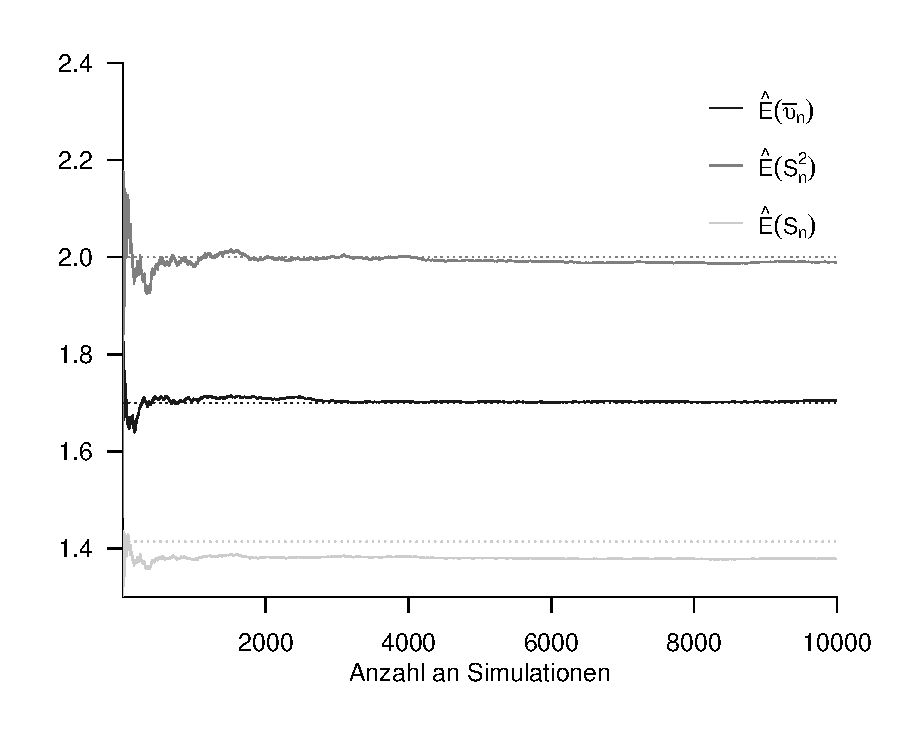
\includegraphics[width=0.75\linewidth]{10_Abbildungen/wtfi_10_bias} \end{center}
\end{frame}

\begin{frame}{\small Schätzereigenschaften bei endlichen Stichproben
\textbar{} Varianz und Standardfehler}
\protect\hypertarget{schuxe4tzereigenschaften-bei-endlichen-stichproben-varianz-und-standardfehler}{}
\small
\begin{definition}[Varianz und Standardfehler]
$\ups := \ups_1,...,\ups_n \sim  p_\theta$ sei eine Stichprobe und $\hat{\tau}_n$ sei ein Schätzer von $\tau$.
\begin{itemize}
\item Die \textit{Varianz} von $\hat{\tau}_n$ ist definiert als
\begin{equation}
\mathbb{V}_\theta(\hat{\tau}_n) :=
\mathbb{E}_\theta
\left((\hat{\tau}_n(\ups) - \mathbb{E}_\theta(\hat{\tau}_n(\ups)))^2\right).
\end{equation}
\item Der \textit{Standardfehler} von $\hat{\tau}_n$ ist definiert als
\begin{equation}
\mbox{SE}(\hat{\tau}_n) := \sqrt{\mathbb{V}_\theta(\hat{\tau}_n)}
\end{equation}
\end{itemize}
\end{definition}

Bemerkungen

\begin{itemize}
\tightlist
\item
  Die Varianz eines Schätzers \(\hat{\tau}_n\) ist die Varianz der
  Zufallsvariable \(\hat{\tau}_n(\ups)\).
\item
  Der Standardfehler eines Schätzers \(\hat{\tau}_n\) ist die
  Standardabweichung von \(\hat{\tau}_n(\ups)\).
\end{itemize}
\end{frame}

\begin{frame}{\small Schätzereigenschaften bei endlichen Stichproben
\textbar{} Varianz und Standardfehler}
\protect\hypertarget{schuxe4tzereigenschaften-bei-endlichen-stichproben-varianz-und-standardfehler-1}{}
\small
\begin{theorem}[Standardfehler des Stichprobenmittels]
\justifying
\normalfont
$\ups := \ups_1,...,\ups_n \sim p_\theta$ sei die Stichprobe eines parametrischen
statistischen Produktmodells. Dann ist der \textit{Standardfehler des Stichprobenmittels} gegeben durch
\begin{equation}
\mbox{SE}(\bar{\ups}_n) = \frac{\mathbb{S}_\theta(\ups_1)}{\sqrt{n}}.
\end{equation}
Der Standardfehler des Stichprobenmittels heißt auch \textit{Standardfehler des Mittelwertes}.
\end{theorem}

\footnotesize

\underline{Beweis}

Per definitionem und mit
\(\mathbb{V}_\theta(\bar{\ups}_n) = \mathbb{V}_\theta(\ups_1)/n\),
ergibt sich \begin{equation}
\mbox{SE}(\bar{\ups}_n)
= \sqrt{\mathbb{V}_\theta(\bar{\ups}_n)}
= \sqrt{\frac{\mathbb{V}_\theta(\ups_1)}{n}}
= \frac{\mathbb{S}_\theta(\ups_1)}{\sqrt{n}}.
\end{equation}

Bemerkungen

\begin{itemize}
\tightlist
\item
  Der Standardfehler des Mittelwerts beschreibt die Variabilität des
  Stichprobenmittels.
\item
  Da \(\mathbb{S}_\theta(\ups_1)\) unbekannt ist, ist auch
  \(\mbox{SE}(\bar{\ups}_n)\) unbekannt.
\item
  Ein verzerrter Schätzer für den Standardfehler des Stichprobenmittels
  ist gegeben durch
  \(\hat{\mbox{SE}}(\bar{\ups}_n) = \frac{s_n}{\sqrt{n}}\).
\end{itemize}
\end{frame}

\begin{frame}{\small Schätzereigenschaften bei endlichen Stichproben
\textbar{} Varianz und Standardfehler}
\protect\hypertarget{schuxe4tzereigenschaften-bei-endlichen-stichproben-varianz-und-standardfehler-2}{}
Beispiel (Standardfehler des Bernoulli Parameter Maximum-Likelihood
Schätzes)

\small

Es sei \(\ups := \ups_1,...,\ups_n \sim \mbox{Bern}(\mu)\) und
\(\hat{\mu}^{\mbox{\tiny ML}}_n\) der Maximum-Likelihood Schätzer für
\(\mu\). Dann ist \begin{equation}
\mbox{SE}\left(\hat{\mu}^{\mbox{\tiny ML}}_n\right) = \sqrt{\frac{\mu(1-\mu)}{n}}.
\end{equation}

\footnotesize

\underline{Beweis}

Es gilt \tiny \begin{align}
\begin{split}
\mbox{SE}\left(\hat{\mu}^{\mbox{\tiny ML}}_n\right)
= \sqrt{\mathbb{V}_\mu\left(\hat{\mu}^{\mbox{\tiny ML}}_n\right)}
& = \sqrt{\mathbb{V}_\mu\left(\frac{1}{n}\sum_{i=1}^n \ups_i \right)} \\
& = \sqrt{\frac{1}{n^2}\sum_{i=1}^n \mathbb{V}_\mu(\ups_i)}
= \sqrt{\frac{n \mu(1-\mu)}{n^2}}
= \sqrt{\frac{\mu(1-\mu)}{n}},
\end{split}
\end{align} \footnotesize wobei die dritte Gleichung mit der
Unabhängigkeit der \(\ups_i, i = 1,...,n\) und die vierte Gleichung mit
der Varianz
\(\mathbb{V}_\mu(\ups_1) = \mathbb{V}_\mu(\ups_i) = \mu(1-\mu), i = 1,...,n\)
der Bernoulli Stichprobenvariablen folgt.

\footnotesize

Bemerkung \vspace{-1mm}

\begin{itemize}
\tightlist
\item
  Ein Schätzer für den Standardfehler
  \(\mbox{SE}\left(\hat{\mu}^{\mbox{\tiny ML}}_n\right)\) ist
  \(\hat{\mbox{SE}}\left(\hat{\mu}^{\mbox{\tiny ML}}_n\right) = \sqrt{\frac{\hat{\mu}^{\mbox{\tiny ML}}_n(1-\hat{\mu}^{\mbox{\tiny ML}}_n)}{n}}\)
\end{itemize}
\end{frame}

\begin{frame}[fragile]{\small Schätzereigenschaften bei endlichen
Stichproben \textbar{} Varianz und Standardfehler}
\protect\hypertarget{schuxe4tzereigenschaften-bei-endlichen-stichproben-varianz-und-standardfehler-3}{}
\vspace{1mm}
\small

Simulation von \(\ups_1,...,\ups_n \sim \mbox{Bern}(\mu)\) mit
\(\mu = 0.4\) \vspace{1mm}

\tiny
\setstretch{0.9}

\begin{Shaded}
\begin{Highlighting}[]
\CommentTok{\# Modellformulierung}
\NormalTok{mu          }\OtherTok{=} \FloatTok{0.4}                                   \CommentTok{\# wahrer, aber unbekannter, Parameterwert}
\NormalTok{n\_all       }\OtherTok{=} \FunctionTok{c}\NormalTok{(}\DecValTok{20}\NormalTok{,}\DecValTok{100}\NormalTok{,}\DecValTok{200}\NormalTok{)                         }\CommentTok{\# Stichprobengrößen n}
\NormalTok{ns          }\OtherTok{=} \FloatTok{1e4}                                   \CommentTok{\# Anzahl der Simulationen}
\NormalTok{mu\_hat\_ML   }\OtherTok{=} \FunctionTok{matrix}\NormalTok{(}\FunctionTok{rep}\NormalTok{(}\ConstantTok{NaN}\NormalTok{, }\FunctionTok{length}\NormalTok{(n\_all)}\SpecialCharTok{*}\NormalTok{ns),    }\CommentTok{\# Maximum{-}Likelihood Schätzearray}
                     \AttributeTok{nrow =} \FunctionTok{length}\NormalTok{(n\_all))}

\CommentTok{\# Stichprobengroesseniterationen}
\ControlFlowTok{for}\NormalTok{(i }\ControlFlowTok{in} \FunctionTok{seq\_along}\NormalTok{(n\_all))\{}

    \CommentTok{\# Simulationsiterationen}
    \ControlFlowTok{for}\NormalTok{(s }\ControlFlowTok{in} \DecValTok{1}\SpecialCharTok{:}\NormalTok{ns)\{}
\NormalTok{        y               }\OtherTok{=} \FunctionTok{rbinom}\NormalTok{(n\_all[i],}\DecValTok{1}\NormalTok{,mu)     }\CommentTok{\# Stichprobenrealisation von y\_1,...,y\_n}
\NormalTok{        mu\_hat\_ML[i,s]  }\OtherTok{=} \FunctionTok{mean}\NormalTok{(y)                   }\CommentTok{\# Stichprobenmittel}
\NormalTok{    \}}
\NormalTok{\}}
\end{Highlighting}
\end{Shaded}

\vspace{1mm}

\footnotesize

Die Varianz bzw. der Standardfehler von
\(\hat{\mu}^{\mbox{\tiny ML}}_n\) hängen von \(n\) ab.

\begin{center}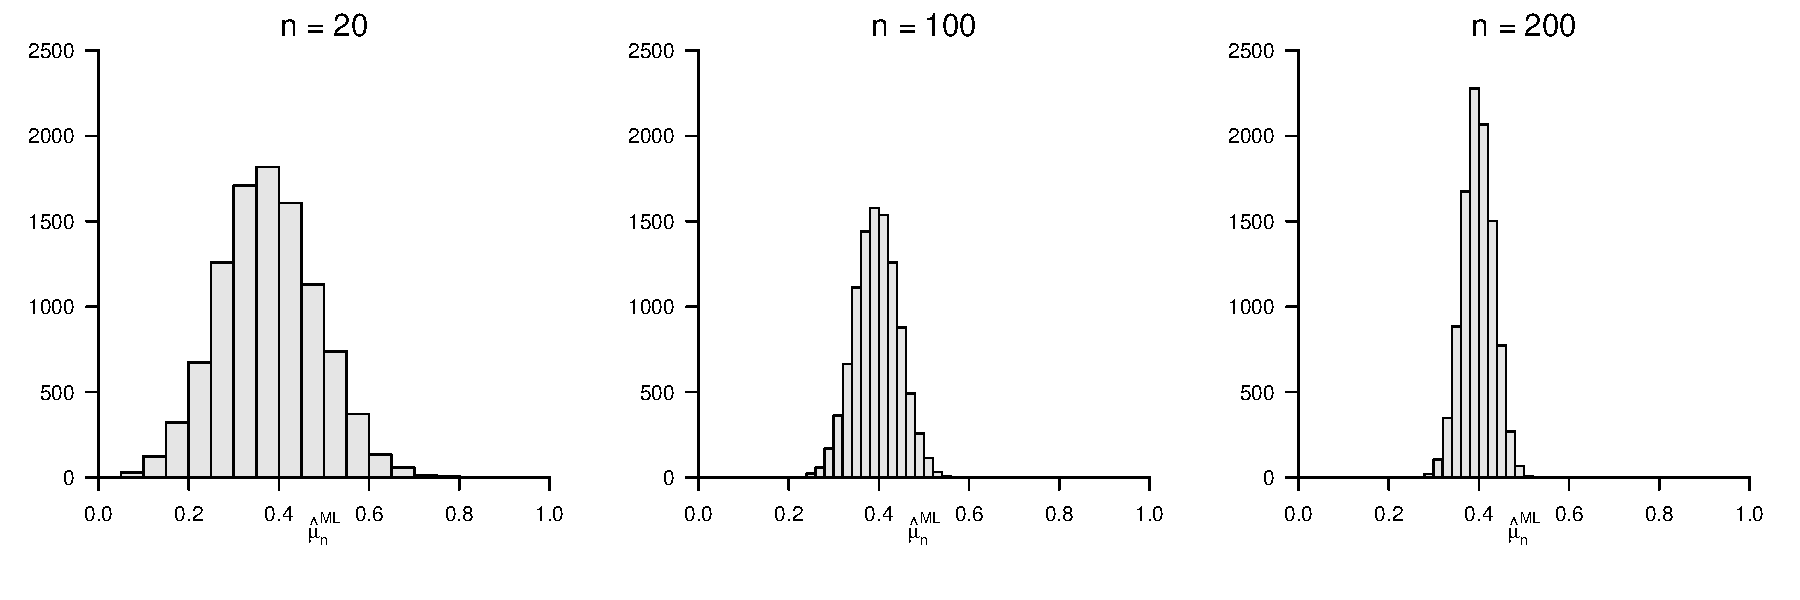
\includegraphics[width=0.9\linewidth]{10_Abbildungen/wtfi_10_sem} \end{center}
\end{frame}

\begin{frame}{\small Schätzereigenschaften bei endlichen Stichproben
\textbar{} Mittlerer quadratischer Fehler}
\protect\hypertarget{schuxe4tzereigenschaften-bei-endlichen-stichproben-mittlerer-quadratischer-fehler}{}
\small
\begin{definition}[Mittlerer quadratischer Fehler]
\justifying
$\ups := \ups_1,...,\ups_n \sim  p_\theta$ sei die Stichprobe eines parametrischen
statistischen Produktmodells $\mathcal{M}$ und $\hat{\tau}_n$ ein Schätzer für $\tau$.
Dann ist der \textit{mittlere quadratischer Fehler (engl. mean squared error)}
von $\hat{\tau}_n$ definiert als
\begin{equation}
\mbox{MQF}(\hat{\tau}_n) := \mathbb{E}_\theta\left((\hat{\tau}_n(\ups) - \tau(\theta))^2\right).
\end{equation}
\end{definition}

\footnotesize

Bemerkungen

\begin{itemize}
\tightlist
\item
  Der MQF von \(\hat{\tau}_n\) ist die erwartete quadrierte Abweichung
  von \(\hat{\tau}_n(\ups)\) von \(\tau(\theta)\).
\item
  Die Varianz von \(\hat{\tau}_n\) ist die erwartete quadrierte
  Abweichung von \(\hat{\tau}_n\) von
  \(\mathbb{E}_\theta(\hat{\tau}_n(\ups))\).
\item
  \(\mathbb{E}_\theta(\hat{\tau}_n(\ups))\) kann mit \(\tau(\theta)\)
  übereinstimmen, muss es aber nicht.
\end{itemize}
\end{frame}

\begin{frame}{\small Schätzereigenschaften bei endlichen Stichproben
\textbar{} Mittlerer quadratischer Fehler}
\protect\hypertarget{schuxe4tzereigenschaften-bei-endlichen-stichproben-mittlerer-quadratischer-fehler-1}{}
\small
\begin{theorem}[Zerlegung des mittleren quadratischen Fehlers]
\justifying
\normalfont
$\ups := \ups_1,...,\ups_n \sim  p_\theta$ sei die Stichprobe eines parametrischen statistischen
Produktmodells $\mathcal{M}$, $\hat{\tau}_n$ sei ein Schätzer für $\tau$, und
$\mbox{MQF}(\hat{\tau}_n)$ sei der mittlere quadratische Fehler von $\hat{\tau}_n$.
Dann gilt
\begin{equation}
\mbox{MQF}(\hat{\tau}_n) = \mbox{B}(\hat{\tau}_n)^2 + \mathbb{V}_\theta(\hat{\tau}_n).
\end{equation}
\end{theorem}

\footnotesize

Bemerkungen

\begin{itemize}
\tightlist
\item
  MQF = Bias\(^2\) + Varianz.
\item
  Der MQF kann als Bias-Varianz Abwägungskriterium benutzt werden.
\item
  Kleine Schätzerverzerrungen können gegenüber einer großen
  Schätzervarianz präferiert werden.
\end{itemize}
\end{frame}

\begin{frame}{\small Schätzereigenschaften bei endlichen Stichproben
\textbar{} Mittlerer quadratischer Fehler}
\protect\hypertarget{schuxe4tzereigenschaften-bei-endlichen-stichproben-mittlerer-quadratischer-fehler-2}{}
\footnotesize

\underline{Beweis}

Zur Vereinfachung der Notation seien \(\tau := \tau(\theta)\),
\(\hat{\tau}_n := \hat{\tau}_n(\ups)\) und
\(\bar{\tau}_n := \mathbb{E}_\theta(\hat{\tau}_n(\ups))\). Dann gilt:
\begin{align*}
\begin{split}
\mathbb{E}_\theta\left((\hat{\tau}_n - \tau)^2\right)
& = \mathbb{E}_\theta\left((\hat{\tau}_n - \bar{\tau}_n + \bar{\tau}_n - \tau)^2\right) \\
& = \mathbb{E}_\theta
\left(
(\hat{\tau}_n - \bar{\tau}_n)^2
+ 2(\hat{\tau}_n - \bar{\tau}_n)(\bar{\tau}_n - \tau)
+ (\bar{\tau}_n - \tau)^2
\right)
\\
& = \mathbb{E}_\theta\left((\hat{\tau}_n - \bar{\tau}_n)^2\right)
+ 2\mathbb{E}_\theta\left((\hat{\tau}_n - \bar{\tau}_n)(\bar{\tau}_n - \tau)\right)
+ \mathbb{E}_\theta\left((\bar{\tau}_n - \tau)^2\right) \\
& = \mathbb{E}_\theta\left((\hat{\tau}_n - \bar{\tau}_n)^2\right)
+ 2\mathbb{E}_\theta\left(
\hat{\tau}_n\bar{\tau}_n - \hat{\tau}_n\tau
- \bar{\tau}_n\bar{\tau}_n + \bar{\tau}_n\tau
\right)
+ \mathbb{E}_\theta\left((\bar{\tau}_n - \tau)^2\right)
\\
& =
\mathbb{E}_\theta\left((\hat{\tau}_n - \bar{\tau}_n)^2\right)
+ 2\left(
\bar{\tau}_n\bar{\tau}_n - \bar{\tau}_n\tau
\right)
+ \mathbb{E}_\theta\left((\bar{\tau}_n - \tau)^2\right) \\
& =
\mathbb{E}_\theta\left((\hat{\tau}_n - \bar{\tau}_n)^2\right)
+ 0
+ \mathbb{E}_\theta\left((\bar{\tau}_n - \tau)^2\right) \\
& =
\mathbb{E}_\theta\left((\bar{\tau}_n - \tau)^2\right)
+ \mathbb{E}_\theta\left((\hat{\tau}_n - \bar{\tau}_n)^2\right) \\
& =
\mathbb{E}_\theta\left((\mathbb{E}_\theta(\hat{\tau}_n) - \tau)^2\right)
+ \mathbb{E}_\theta\left((\hat{\tau}_n - \mathbb{E}_\theta(\hat{\tau}_n))^2\right) \\
& =
(\mathbb{E}_\theta(\hat{\tau}_n) - \tau)^2
+ \mathbb{V}_\theta(\hat{\tau}_n) \\
& =
\mbox{B}(\hat{\tau}_n)^2
+ \mathbb{V}_\theta(\hat{\tau}_n).
\end{split}
\end{align*}
\end{frame}

\begin{frame}{}
\protect\hypertarget{section-10}{}
\large
\vfill
\setstretch{2.3}

Grundbegriffe

Maximum-Likelihood Schätzer

Schätzereigenschaften bei endlichen Stichproben

\textbf{Asymptotische Schätzereigenschaften}

Eigenschaften von Maximum-Likelihood Schätzern

Selbstkontrollfragen \vfill
\end{frame}

\begin{frame}{Asymptotische Schätzereigenschaften}
\protect\hypertarget{asymptotische-schuxe4tzereigenschaften}{}
\setstretch{1.8}

Vorbemerkungen zu Asymptotischen Schätzereigenschaften \small

Dieser Abschnitt ist eine Kurzeinführung in die
\textit{Asymptotische Statistik (AS)}.

Die AS befasst sich mit dem Verhalten von Statistiken bei großen
Stichproben.

Methoden der AS werden benutzt, um

\begin{itemize}
\tightlist
\item
  qualitative Schätzereigenschaften zu studieren und
\item
  Schätzereigenschaften für große Stichprobengrößen zu approximieren.
\end{itemize}

Moderne Stichproben sind üblicherweise groß.

Die Methoden der AS sind also praktisch einsetzbar und gerechtfertigt.

Vaart (1998) gibt eine ausführliche Einführung in die AS.
\end{frame}

\begin{frame}{Asymptotische Schätzereigenschaften}
\protect\hypertarget{asymptotische-schuxe4tzereigenschaften-1}{}
Asymptotische Schätzereigenschaften

\footnotesize

Wir betrachten vier asymptotische Schätzereigenschaften.

\begin{enumerate}
[(1)]
\tightlist
\item
  Asymptotische Erwartungstreue
\item
  Konsistenz
\item
  Asymptotische Normalverteilung
\item
  Asymptotische Effizienz
\end{enumerate}

Intuitiv haben diese folgende Bedeutungen:

\begin{enumerate}
[(1)]
\item
  \justifying Ein Schätzer \(\hat{\tau}_n\) für \(\tau\) heißt
  \emph{asymptotisch erwartungstreu}, wenn der Erwartungswert von
  \(\hat{\tau}_n\) für große Stichprobengrößen \(n \to \infty\) gleich
  dem wahren, aber unbekannten, Wert \(\tau(\theta)\) ist.
\item
  Ein Schätzer \(\hat{\tau}_n\) für \(\tau\) heißt \emph{konsistent},
  wenn für große Stichprobengrößen \(n \to \infty\) die
  Wahrscheinlichkeit dafür, dass \(\hat{\tau}_n(\ups)\) vom wahren, aber
  unbekannten, Wert \(\tau(\theta)\) abweicht beliebig klein wird.
\item
  Ein Schätzer \(\hat{\tau}_n\) für \(\tau\) heißt \emph{asymptotisch
  normalverteilt}, wenn für große Stichprobengrößen \(n \to \infty\),
  die Verteilung von \(\hat{\tau}_n\) durch eine Normalverteilung
  gegeben ist.
\item
  Ein Schätzer \(\hat{\tau}_n\) für \(\tau\) heißt \emph{asymptotisch
  effizient}, wenn für große Stichprobengrößen \(n \to \infty\) die
  Verteilung von \(\hat{\tau}_n\) durch eine Normalverteilung mit
  Erwartungswertparameter \(\tau(\theta)\) und Varianzparameter gleich
  der Cramér-Rao-Schranke gegeben ist. Wir vertiefen die asymptotische
  Effienz in einem Appendix.
\end{enumerate}
\end{frame}

\begin{frame}{\small Asymptotische Schätzereigenschaften \textbar{}
Asymptotische Erwartungstreue}
\protect\hypertarget{asymptotische-schuxe4tzereigenschaften-asymptotische-erwartungstreue}{}
\small
\begin{definition}[Asymptotische Erwartungstreue]
\justifying
$\ups := \ups_1,...,\ups_n \sim p_\theta$ sei die Stichprobe eines parametrischen statistischen
Produktmodells $\mathcal{M}$ und  $\hat{\tau}_n$ sei ein Schätzer für $\tau$.
$\hat{\tau}_n$ heißt \textit{asymptotisch erwartungstreu}, wenn
\begin{equation}
\lim_{n\to\infty} \mathbb{E}_\theta(\hat{\tau}_n(\ups)) = \tau(\theta) \mbox{ für alle }
\theta \in \Theta.
\end{equation}
\end{definition}

\footnotesize

Bemerkungen

\begin{itemize}
\tightlist
\item
  Asymptotisch erwartungstreue Schätzer sind für ``unendlich große''
  Stichproben erwartungstreu.
\item
  Erwartungstreue Schätzer sind immer auch asymptotisch erwartungstreu.
\end{itemize}
\end{frame}

\begin{frame}{\small Asymptotische Schätzereigenschaften \textbar{}
Asymptotische Erwartungstreue}
\protect\hypertarget{asymptotische-schuxe4tzereigenschaften-asymptotische-erwartungstreue-1}{}
\footnotesize
\begin{theorem}[Asymptotische Erwartungstreue des Varianzparameterschätzers] 
\justifying
\normalfont
Es sei $\ups := \ups_1,...,\ups_n \sim N(\mu,\sigma^2)$. Dann ist der Maximum-Likelihood
Schätzer des Varianzparameters,
\begin{equation}
\hat{\sigma}_n^{2^{\mbox{\tiny ML}}}
:= \frac{1}{n}\sum_{i=1}^n \left(\ups_i - \bar{\ups}_n \right)^2
\end{equation}
asymptotisch erwartungstreu.
\end{theorem}

\underline{Beweis}

Mit der Erwartungstreue der Stichprobenvarianz ergibt sich\\
\tiny \begin{align*}
\begin{split}
\mathbb{E}_{\mu,\sigma^2}\left(\hat{\sigma}_n^{2^{\mbox{\tiny ML}}} \right)
= \mathbb{E}_{\mu,\sigma^2}\left(\frac{1}{n}\sum_{i=1}^n \left(\ups_i - \bar{\ups}_n \right)^2 \right)
= \frac{1}{n}\mathbb{E}_{\mu,\sigma^2}\left(\sum_{i=1}^n \left(\ups_i - \bar{\ups}_n \right)^2 \right)
=    \frac{n-1}{n}\sigma^2 \\
\end{split}
\end{align*} \footnotesize Also gilt
\(\mathbb{E}_{\mu,\sigma^2}\left(\hat{\sigma}_n^{2^{\mbox{\tiny ML}}} \right) \neq \sigma^2\).
\(\hat{\sigma}_n^{2^{\mbox{\tiny ML}}}\) ist also ein verzerrter
Schätzer von \(\sigma^2\). Allerdings gilt \((n-1)/n \to 1\) für
\(n \to \infty\), so dass \begin{equation}
\lim_{n \to \infty} \mathbb{E}_{\mu,\sigma^2}\left(\hat{\sigma}_n^{2^{\mbox{\tiny ML}}}\right) =
\lim_{n \to \infty}  \frac{n-1}{n}\sigma^2 =
\sigma^2 \lim_{n \to \infty}  \frac{n-1}{n} =
\sigma^2.
\end{equation}
\end{frame}

\begin{frame}[fragile]{\small Asymptotische Schätzereigenschaften
\textbar{} Asymptotische Erwartungstreue}
\protect\hypertarget{asymptotische-schuxe4tzereigenschaften-asymptotische-erwartungstreue-2}{}
\small

Simulation von \(\ups_1,...,\ups_n \sim N(\mu,\sigma^2)\) mit
\(\mu = 1\), \(\sigma^2 = 2\)

\footnotesize
\setstretch{1}
\vspace{2mm}

\begin{Shaded}
\begin{Highlighting}[]
\CommentTok{\# Modellformulierung}
\NormalTok{mu        }\OtherTok{=} \DecValTok{1}                       \CommentTok{\# wahrer, aber unbekannter, Erwartungswertparameter}
\NormalTok{sigsqr    }\OtherTok{=} \DecValTok{2}                       \CommentTok{\# wahrer, aber unbekannter, Varianzparameter}
\NormalTok{n         }\OtherTok{=} \FunctionTok{seq}\NormalTok{(}\DecValTok{1}\NormalTok{,}\DecValTok{100}\NormalTok{, }\AttributeTok{by =} \DecValTok{2}\NormalTok{)      }\CommentTok{\# Stichprobengroessen}
\NormalTok{ns        }\OtherTok{=} \FloatTok{1e3}                     \CommentTok{\# Anzahl Simulation pro Stichprobengroesse}
\NormalTok{sigsqr\_ml }\OtherTok{=} \FunctionTok{matrix}\NormalTok{(                 }\CommentTok{\# \textbackslash{}hat\{\textbackslash{}sigma\^{}2\}\^{}\{ML\} Array}
            \FunctionTok{rep}\NormalTok{(}\ConstantTok{NaN}\NormalTok{, }\FunctionTok{length}\NormalTok{(n)}\SpecialCharTok{*}\NormalTok{ns),}
            \AttributeTok{ncol =} \FunctionTok{length}\NormalTok{(n))}

\CommentTok{\# Stichprobengroesseniterationen}
\ControlFlowTok{for}\NormalTok{(i }\ControlFlowTok{in} \FunctionTok{seq\_along}\NormalTok{(n))\{}

    \CommentTok{\# Simulationsiterationen}
    \ControlFlowTok{for}\NormalTok{(s }\ControlFlowTok{in} \DecValTok{1}\SpecialCharTok{:}\NormalTok{ns)\{}

        \CommentTok{\# Stichprobenrealisation}
\NormalTok{        y               }\OtherTok{=} \FunctionTok{rnorm}\NormalTok{(n[i], mu, }\FunctionTok{sqrt}\NormalTok{(sigsqr))}

        \CommentTok{\# \textbackslash{}hat\{\textbackslash{}sigma\^{}2\}\^{}\{ML\}}
\NormalTok{        sigsqr\_ml[s,i]  }\OtherTok{=}\NormalTok{ ((n[i]}\SpecialCharTok{{-}}\DecValTok{1}\NormalTok{)}\SpecialCharTok{/}\NormalTok{n[i])}\SpecialCharTok{*}\FunctionTok{var}\NormalTok{(y)}
\NormalTok{    \}}
\NormalTok{\}}
\NormalTok{E\_sigsqr\_ml }\OtherTok{=} \FunctionTok{colMeans}\NormalTok{(sigsqr\_ml)   }\CommentTok{\# Erwartungswertschaetzung}
\end{Highlighting}
\end{Shaded}
\end{frame}

\begin{frame}{\small Asymptotische Schätzereigenschaften \textbar{}
Asymptotische Erwartungstreue}
\protect\hypertarget{asymptotische-schuxe4tzereigenschaften-asymptotische-erwartungstreue-3}{}
\small

Simulation \(\ups_1,...,\ups_n \sim N(\mu,\sigma^2)\) mit \(\mu = 1\),
\(\sigma^2 = 2\) \vspace{2mm}

\begin{center}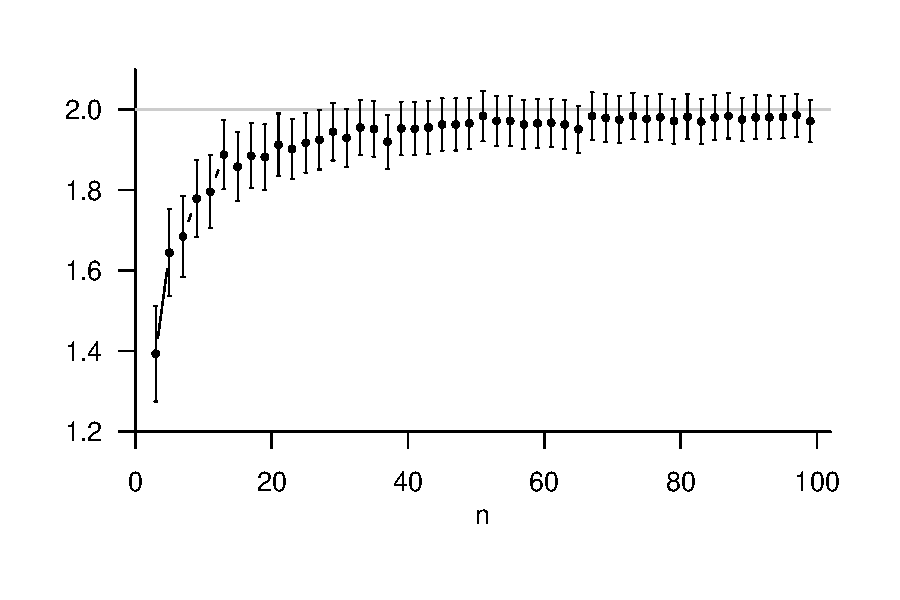
\includegraphics[width=0.85\linewidth]{10_Abbildungen/wtfi_10_sigsqr_ml} \end{center}
\end{frame}

\begin{frame}{\small Asymptotische Schätzereigenschaften \textbar{}
Konsistenz}
\protect\hypertarget{asymptotische-schuxe4tzereigenschaften-konsistenz}{}
\small
\begin{definition}[Konsistenz]
\justifying
$\ups := \ups_1,...,\ups_n \sim p_\theta$ sei die Stichprobe eines parametrischen statistischen
Produktmodells $\mathcal{M}$ und $\hat{\tau}_n$ sei ein Schätzer von $\tau$. Eine
Folge von Schätzern $\hat{\tau}_1, \hat{\tau}_2, ...$ wird dann eine
\textit{konsistente Folge von Schätzern} genannt, wenn für jedes $\epsilon > 0$
und jedes $\theta \in \Theta$ gilt, dass
\begin{equation*}
\lim_{n\to \infty}
\mathbb{P}_\theta\left(|\hat{\tau}_n(\ups) - \tau(\theta)| \ge \epsilon \right) = 0.
\end{equation*}
Wenn $\hat{\tau}_1,\hat{\tau}_2,...$ eine konsistente Folge von Schätzern ist,
dann heißt $\hat{\tau}_n$   \textit{konsistenter Schätzer}.
\end{definition}
\footnotesize

Bemerkungen

\begin{itemize}
\tightlist
\item
  Für \(n \to \infty\) wird die Wahrscheinlichkeit, dass
  \(\hat{\tau}_n(\ups)\) beliebig nah bei \(\tau(\theta)\) liegt, groß.
\item
  Für \(n \to \infty\) wird die Wahrscheinlichkeit, dass
  \(\hat{\tau}_n(\ups)\) von \(\tau(\theta)\) abweicht, klein.
\item
  Diese Eigenschaften gelten für alle möglichen wahren, aber
  unbekannten, Parameterwerte.
\item
  Die Konvergenz ist \textit{Konvergenz in Wahrscheinlichkeit}.
\item
  Konsistenz von Schätzern kann direkt oder mit Kriterien nachgewiesen
  werden.
\end{itemize}
\end{frame}

\begin{frame}{\small Asymptotische Schätzereigenschaften \textbar{}
Konsistenz}
\protect\hypertarget{asymptotische-schuxe4tzereigenschaften-konsistenz-1}{}
\small
\begin{theorem}[Mittlerer-Quadratischer-Fehler-Kriterium für Konsistenz]
\normalfont
\justifying
$\ups := \ups_1,...,\ups_n \sim p_\theta$ sei die Stichprobe eines parametrischen statistischen
Produktmodells $\mathcal{M}$ und $\hat{\tau}_n$ sei ein Schätzer von $\tau$. Wenn
$\lim_{n\to \infty} \mbox{MQF}(\hat{\tau}_n) = 0$ gilt, dann ist $\hat{\tau}_n$
ein konsistenter Schätzer.
\end{theorem}

\footnotesize

\underline{Beweis}

Mit der Chebychev-Ungleichung gilt, dass \begin{equation}
\mathbb{P}_\theta\left(|\hat{\tau}_n(\ups) - \tau(\theta)| \ge \epsilon \right) \le
\frac{\mathbb{E}_\theta\left((\hat{\tau}_n(\ups) -  \tau(\theta))^2\right)}{\epsilon^2}
\end{equation} Grenzwertbildung ergibt dann \begin{equation}
\lim_{n\to \infty}\mathbb{P}_\theta\left(|\hat{\tau}_n(\ups) - \tau(\theta)| \ge \epsilon \right) \le
\frac{1}{\epsilon^2}\lim_{n\to\infty}\mathbb{E}_\theta\left((\hat{\tau}_n(\ups) - \tau(\theta))^2\right).
\end{equation} Wenn also
\(\lim_{n\to\infty}\mathbb{E}_\theta\left((\hat{\tau}_n(\ups) - \tau(\theta))^2\right) = 0\)
gilt, dann gilt mit
\(\mathbb{P}_\theta(|\hat{\tau}_n(\ups) - \tau(\theta)| \ge \epsilon)\ge 0\),
dass \begin{equation}
\lim_{n\to \infty}\mathbb{P}_\theta\left(|\hat{\tau}_n(\ups) - \tau(\theta)| \ge \epsilon \right) = 0.
\end{equation} Also ist \(\hat{\tau}_n\) ein konsistenter Schätzer.
\end{frame}

\begin{frame}{\small Asymptotische Schätzereigenschaften \textbar{}
Konsistenz}
\protect\hypertarget{asymptotische-schuxe4tzereigenschaften-konsistenz-2}{}
\small
\begin{theorem}[Bias-Varianz-Kriterium für Konsistenz]
\normalfont
\justifying
$\ups_1,...,\ups_n \sim p_\theta$ sei die Stichprobe eines parametrischen statistischen
Produktmodells $\mathcal{M}$ und $\hat{\tau}_n$ sei ein Schätzer von $\tau$. Wenn
\begin{equation}
\lim_{n\to \infty} \mbox{B}(\hat{\tau}_n) = 0
\mbox{ und }
\lim_{n\to \infty} \mathbb{V}_\theta(\hat{\tau}_n) = 0
\end{equation}
gilt, dann ist $\hat{\tau}_n$ ein konsistenter Schätzer
\end{theorem}
\footnotesize

\underline{Beweis}

Wenn \(n \to \infty\), dann gilt \(\mbox{B}(\hat{\tau}_n) \to 0\), also
auch \(\mbox{B}(\hat{\tau}_n)^2 \to 0\). Wenn für \(n \to \infty\)
sowohl \(\mbox{B}(\hat{\tau}_n)^2 \to 0\) als auch
\(\mathbb{V}_\theta(\hat{\tau}_n) \to 0\), dann gilt auch
\(\lim_{n\to \infty} \mbox{MQF}(\hat{\theta}_n) = 0\). Also gilt mit dem
MQF-Kriterium, dass \(\hat{\tau}_n\) konsistent ist.
\end{frame}

\begin{frame}{\small Asymptotische Schätzereigenschaften \textbar{}
Konsistenz}
\protect\hypertarget{asymptotische-schuxe4tzereigenschaften-konsistenz-3}{}
\small
\begin{theorem}[Konsistenz des Erwartungswertschätzers bei Normalverteilung] 
\justifying
\normalfont
Es sei $\ups := \ups_1,...,\ups_n \sim N(\mu,\sigma^2)$. Dann ist $\bar{\ups}_n$
ein konsistenter Schätzer von $\mathbb{E}(\ups_1)$.
\end{theorem}
\footnotesize

\underline{Beweis}

Mit der Erwartungstreue des Stichprobenmittels als Schätzer für den
Erwartungswert gilt zunächst \begin{equation}
\lim_{n \to \infty} \mbox{B}(\bar{\ups}_n) =  0
\end{equation} Weiterhin gilt mit der Varianz des Stichprobenmittels
\begin{equation}
\lim_{n \to \infty} \mathbb{V}_\theta(\bar{\ups}_n) = \lim_{n\to \infty} \frac{1}{n}\mathbb{V}(\ups_1) = 0.
\end{equation} Mit dem Bias-Varianz-Kriterium folgt dann die Konsistenz
von \(\bar{\ups}_n\) als Schätzer von \(\mathbb{E}(\ups_1)\)
\end{frame}

\begin{frame}[fragile]{\small Asymptotische Schätzereigenschaften
\textbar{} Konsistenz}
\protect\hypertarget{asymptotische-schuxe4tzereigenschaften-konsistenz-4}{}
\small

Simulation \(\bar{\ups}_n\) bei
\(\ups_1,...,\ups_n \sim N(\mu,\sigma^2)\) mit \(\mu = 1\),
\(\sigma^2 = 2\)

\footnotesize
\setstretch{.9}
\vspace{1mm}

\begin{Shaded}
\begin{Highlighting}[]
\CommentTok{\# Modellformulierung}
\NormalTok{mu      }\OtherTok{=} \DecValTok{1}                                         \CommentTok{\# w.a.u \textbackslash{}mu Wert}
\NormalTok{sigsqr  }\OtherTok{=} \DecValTok{2}                                         \CommentTok{\# w.a.u. \textbackslash{}sigma\^{}2 Wert}
\NormalTok{n       }\OtherTok{=} \FunctionTok{seq}\NormalTok{(}\DecValTok{1}\NormalTok{,}\FloatTok{1e3}\NormalTok{,}\AttributeTok{by =} \DecValTok{10}\NormalTok{)                        }\CommentTok{\# Stichprobengroesse n}
\NormalTok{eps     }\OtherTok{=} \FunctionTok{c}\NormalTok{(}\FloatTok{0.15}\NormalTok{, }\FloatTok{0.10}\NormalTok{, }\FloatTok{0.05}\NormalTok{)                       }\CommentTok{\# \textbackslash{}epsilon Werte}
\NormalTok{ne      }\OtherTok{=} \FunctionTok{length}\NormalTok{(eps)                               }\CommentTok{\# Anzahl \textbackslash{}epsilon Werte}
\NormalTok{nn      }\OtherTok{=} \FunctionTok{length}\NormalTok{(n)                                 }\CommentTok{\# Anzahl Stichprobengroessen}
\NormalTok{ns      }\OtherTok{=} \FloatTok{1e3}                                       \CommentTok{\# Anzahl Simulationen}
\NormalTok{E       }\OtherTok{=} \FunctionTok{array}\NormalTok{(}\FunctionTok{rep}\NormalTok{(}\ConstantTok{NaN}\NormalTok{,nn,ne,ns),                  }\CommentTok{\# Ereignisindikatorarray}
                \AttributeTok{dim =} \FunctionTok{c}\NormalTok{(nn,ne,ns))}

\CommentTok{\# Simulation}
\ControlFlowTok{for}\NormalTok{(e }\ControlFlowTok{in} \FunctionTok{seq\_along}\NormalTok{(eps))\{                           }\CommentTok{\# \textbackslash{}epsilon Iterationen}
    \ControlFlowTok{for}\NormalTok{(i }\ControlFlowTok{in} \FunctionTok{seq\_along}\NormalTok{(n))\{                         }\CommentTok{\# n Iterationen}
        \ControlFlowTok{for}\NormalTok{(s }\ControlFlowTok{in} \DecValTok{1}\SpecialCharTok{:}\NormalTok{ns)\{                             }\CommentTok{\# Simulationsiterationen}

            \CommentTok{\# Stichprobenrealisationen}
\NormalTok{            y   }\OtherTok{=} \FunctionTok{rnorm}\NormalTok{(n[i], mu, }\FunctionTok{sqrt}\NormalTok{(sigsqr))}
            \ControlFlowTok{if}\NormalTok{(}\FunctionTok{abs}\NormalTok{(}\FunctionTok{mean}\NormalTok{(y) }\SpecialCharTok{{-}}\NormalTok{ mu) }\SpecialCharTok{\textgreater{}=}\NormalTok{ eps[e])\{        }\CommentTok{\# |X\_bar {-} \textbackslash{}mu)| \textbackslash{}ge \textbackslash{}epsilon}
\NormalTok{                E[i,e,s] }\OtherTok{=} \DecValTok{1}
\NormalTok{            \} }\ControlFlowTok{else}\NormalTok{ \{                                }\CommentTok{\# |X\_bar {-} \textbackslash{}mu)| \textless{} \textbackslash{}epsilon}
\NormalTok{                E[i,e,s] }\OtherTok{=} \DecValTok{0}
\NormalTok{            \}}
\NormalTok{        \}}
\NormalTok{    \}}
\NormalTok{\}}

\CommentTok{\# Schaetzung von \textbackslash{}mathbb\{P\}(|\textbackslash{}hat\{\textbackslash{}tau\}\_n(\textbackslash{}ups){-}\textbackslash{}tau(\textbackslash{}theta)| \textbackslash{}ge \textbackslash{}epsilon)}
\NormalTok{P\_hat       }\OtherTok{=} \FunctionTok{apply}\NormalTok{(E, }\FunctionTok{c}\NormalTok{(}\DecValTok{1}\NormalTok{,}\DecValTok{2}\NormalTok{), mean)}
\end{Highlighting}
\end{Shaded}
\end{frame}

\begin{frame}{\small Asymptotische Schätzereigenschaften \textbar{}
Konsistenz}
\protect\hypertarget{asymptotische-schuxe4tzereigenschaften-konsistenz-5}{}
\small

Simulation \(\bar{\ups}_n\) bei
\(\ups_1,...,\ups_n \sim N(\mu,\sigma^2)\) mit \(\mu = 1\),
\(\sigma^2 = 2\)

\begin{center}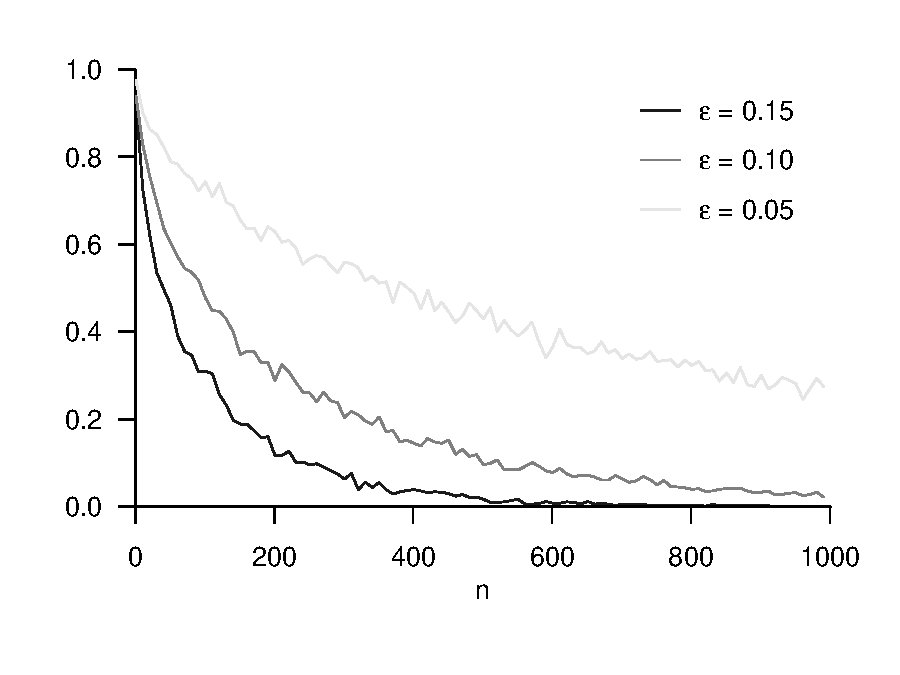
\includegraphics[width=0.8\linewidth]{10_Abbildungen/wtfi_10_konsistenz} \end{center}
\end{frame}

\begin{frame}{\small Asymptotische Schätzereigenschaften \textbar{}
Asymptotische Normalität}
\protect\hypertarget{asymptotische-schuxe4tzereigenschaften-asymptotische-normalituxe4t}{}
\small
\begin{definition}[Asymptotische Normalität]
\justifying
$\ups_1,...,\ups_n \sim p_\theta$ sei die Stichprobe eines parametrischen statistischen
Produktmodells $\mathcal{M}$ und $\hat{\theta}_n$ sei ein Parameterschätzer für
$\theta$. Weiterhin sei $\tilde{\theta} \sim N(\mu,\sigma^2)$ eine normalverteilte
Zufallsvariable mit Erwartungswertparameter $\mu$ und Varianzparameter $\sigma^2$.
Wenn $\hat{\theta}_n$ in Verteilung gegen $\tilde{\theta}$ konvergiert, dann heißt
$\hat{\theta}_n$ \textit{asymptotisch normalverteilt} und wir schreiben
\begin{equation}
\hat{\theta}_n  \stackrel{a}{\sim}  N(\mu,\sigma^2).
\end{equation}
\end{definition}

\footnotesize

Bemerkung

\begin{itemize}
\tightlist
\item
  Konvergenz in Verteilung heißt
  \(\lim_{n\to \infty} P_n(\hat{\theta}_n) = P(\tilde{\theta})\).
\end{itemize}
\end{frame}

\begin{frame}{}
\protect\hypertarget{section-11}{}
\large
\vfill
\setstretch{2.3}

Grundbegriffe

Maximum-Likelihood Schätzer

Schätzereigenschaften bei endlichen Stichproben

Asymptotische Schätzereigenschaften

\textbf{Eigenschaften von Maximum-Likelihood Schätzern}

Selbstkontrollfragen \vfill
\end{frame}

\begin{frame}{Eigenschaften von Maximum-Likelihood Schätzern}
\protect\hypertarget{eigenschaften-von-maximum-likelihood-schuxe4tzern}{}
\setstretch{1.4}
\small
\begin{theorem}[Eigenschaften von Maximum-Likelihood Schätzern]
\normalfont
\justifying
$\ups_1,...,\ups_n \sim p_\theta$ sei die Stichprobe eines parametrischen 
statistischen Produktmodells $\mathcal{M}$ und $\hat{\theta}_n^{\mbox{\tiny{ML}}}$ 
sei ein Maximum-Likelihood Schätzer für $\theta$. Dann gilt, dass 
$\hat{\theta}_n^{\mbox{\tiny{ML}}}$
\begin{itemize}
\item[(1)] nicht notwendigerweise erwartungstreu, aber
\item[(2)] konsistent,
\item[(3)] asymptotisch normalverteilt und
\item[(4)] asymptotisch erwartungstreu.
\end{itemize}
\end{theorem}

Bemerkungen

\begin{itemize}
\tightlist
\item
  Maximum-Likelihood Schätzer sind überdies asymptotisch effizient ist.
\item
  Für einen Beweis verweisen wir auf Held and Sabanés Bové (2014),
  Abschnitt 3.4.
\end{itemize}
\end{frame}

\begin{frame}[fragile]{Eigenschaften von Maximum-Likelihood Schätzern}
\protect\hypertarget{eigenschaften-von-maximum-likelihood-schuxe4tzern-1}{}
\small

Simulation der asymptotische Normalverteilung des Maximum-Likelihood
Bernoulliparameterschätzers

\footnotesize

Die Varianz der asymptotischen Normalverteilung ergibt sich dabei aus
der Cramér-Rao Schranke.

\vspace{1mm}
\setstretch{1}

\begin{Shaded}
\begin{Highlighting}[]
\CommentTok{\# Modellformulierung}
\NormalTok{mu          }\OtherTok{=} \FloatTok{0.4}                                           \CommentTok{\# w.a.u. Parameterwert}
\NormalTok{n\_all       }\OtherTok{=} \FunctionTok{c}\NormalTok{(}\FloatTok{1e1}\NormalTok{,}\FloatTok{5e1}\NormalTok{,}\FloatTok{1e2}\NormalTok{)                                }\CommentTok{\# Stichprobengroesse n}
\NormalTok{ns          }\OtherTok{=} \FloatTok{1e4}                                           \CommentTok{\# Anzahl der Simulationen}
\NormalTok{mu\_hat\_ML   }\OtherTok{=} \FunctionTok{matrix}\NormalTok{(                                       }\CommentTok{\# ML Schaetzerarray}
                        \FunctionTok{rep}\NormalTok{(}\ConstantTok{NaN}\NormalTok{,}
                        \FunctionTok{length}\NormalTok{(n\_all)}\SpecialCharTok{*}\NormalTok{ns),}
                        \AttributeTok{nrow =} \FunctionTok{length}\NormalTok{(n\_all))}
\NormalTok{mu\_hat\_ML\_r }\OtherTok{=} \FloatTok{1e3}                                           \CommentTok{\# ML Schaetzerraumaufloesung}
\NormalTok{mu\_hat\_ML\_y }\OtherTok{=} \FunctionTok{seq}\NormalTok{(}\DecValTok{0}\NormalTok{,}\DecValTok{1}\NormalTok{,}\AttributeTok{len =}\NormalTok{ mu\_hat\_ML\_r)                    }\CommentTok{\# ML Schaetzerraum}
\NormalTok{mu\_hat\_ML\_p }\OtherTok{=} \FunctionTok{matrix}\NormalTok{(}\FunctionTok{rep}\NormalTok{(}\ConstantTok{NaN}\NormalTok{, }\FunctionTok{length}\NormalTok{(n\_all)}\SpecialCharTok{*}\NormalTok{mu\_hat\_ML\_r),   }\CommentTok{\# ML WDF Array}
                     \AttributeTok{nrow =} \FunctionTok{length}\NormalTok{(n\_all))}

\CommentTok{\# Stichprobengroesseniterationen}
\ControlFlowTok{for}\NormalTok{(i }\ControlFlowTok{in} \FunctionTok{seq\_along}\NormalTok{(n\_all))\{}

    \CommentTok{\# Simulationsiterationen}
    \ControlFlowTok{for}\NormalTok{(s }\ControlFlowTok{in} \DecValTok{1}\SpecialCharTok{:}\NormalTok{ns)\{}
\NormalTok{        y               }\OtherTok{=} \FunctionTok{rbinom}\NormalTok{(n\_all[i],}\DecValTok{1}\NormalTok{,mu)             }\CommentTok{\# Stichprobenrealisation}
\NormalTok{        mu\_hat\_ML[i,s]  }\OtherTok{=} \FunctionTok{mean}\NormalTok{(y)                           }\CommentTok{\# ML Schaetzer}
\NormalTok{    \}}

    \CommentTok{\# WDF der asymptotischen Verteilung}
\NormalTok{    mu\_hat\_ML\_p[i,] }\OtherTok{=} \FunctionTok{dnorm}\NormalTok{(mu\_hat\_ML\_y, mu, }\FunctionTok{sqrt}\NormalTok{(mu}\SpecialCharTok{*}\NormalTok{(}\DecValTok{1}\SpecialCharTok{{-}}\NormalTok{mu)}\SpecialCharTok{/}\NormalTok{n\_all[i]))}
\NormalTok{\}}
\end{Highlighting}
\end{Shaded}
\end{frame}

\begin{frame}{Eigenschaften von Maximum-Likelihood Schätzern}
\protect\hypertarget{eigenschaften-von-maximum-likelihood-schuxe4tzern-2}{}
\small

Simulation der asymptotische Normalverteilung des Maximum-Likelihood
Bernoulliparameterschätzers \vspace{10mm}

\begin{center}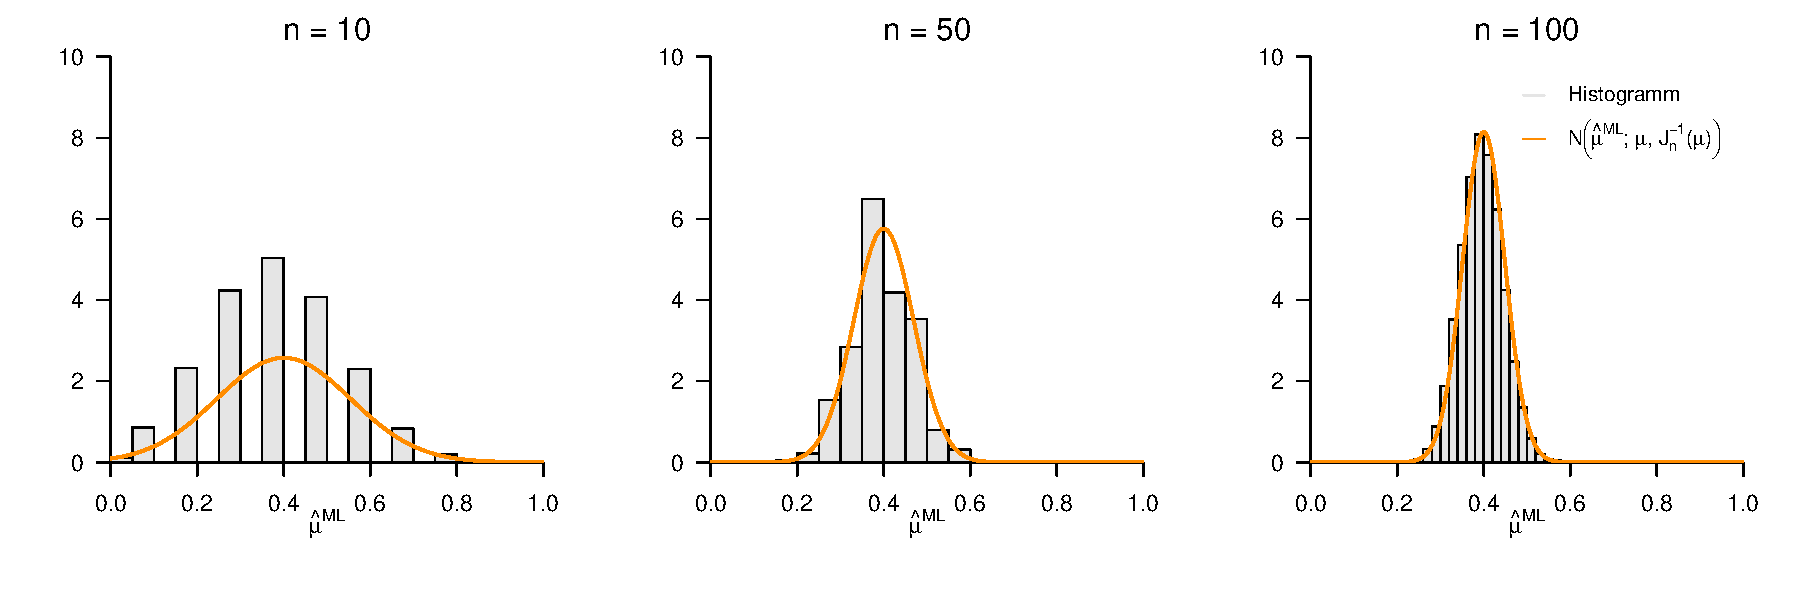
\includegraphics[width=1\linewidth]{10_Abbildungen/wtfi_10_effizienz} \end{center}
\end{frame}

\begin{frame}{}
\protect\hypertarget{section-12}{}
\large
\vfill
\setstretch{2.3}

Grundbegriffe

Maximum-Likelihood Schätzer

Schätzereigenschaften bei endlichen Stichproben

Asymptotische Schätzereigenschaften

Eigenschaften von Maximum-Likelihood Schätzern

\textbf{Selbstkontrollfragen} \vfill
\end{frame}

\begin{frame}{Selbstkontrollfragen}
\protect\hypertarget{selbstkontrollfragen}{}
\footnotesize
\setstretch{1.2}
\begin{enumerate}
\item Definieren und erläutern Sie den Begriff des Parameterpunktschätzers.
\item Definieren Sie die Begriffe der Likelihood-Funktion und der Log-Likelihood Funktion.
\item Definieren Sie den Begriff des Maximum-Likelihood Schätzes.
\item Erläutern Sie das Vorgehen zur Maximum-Likelihood Schätzung für ein parametrisches Produktmodell.
\item Geben Sie den Maximum-Likelihood Schätzer für den Parameter $\mu$ des Bernoullimodells an.
\item Geben Sie den Maximum-Likelihood Schätzer für den Parameter $\mu$ des Normalverteilungmodels an.
\item Geben Sie den Maximum-Likelihood Schätzer für den Parameter $\sigma^2$ des Normalverteilungmodels an.
\item Definieren und erläutern Sie den Begriff der Erwartungstreue eines Schätzers.
\item Definieren Sie die Begriffe der Varianz und des Standardfehlers eines Schätzers.
\item Definieren Sie den Begriff des Mittleren quadratischen Fehlers eines Schätzers.
\item Geben Sie das Theorem zur Zerlegung des Mittleren quadratischen Fehlers wieder.
\item Erläutern Sie den Begriff des asymptotischen Erwartungstreue eines Schätzers
\item Erläutern Sie den Begriff der Konsistenz eines Schätzers.
\item Erläutern Sie den Begriff der asymptotischen Normalität eines Schätzers.
\item Nennen Sie vier Eigenschaften eines Maximum-Likelihood Schätzers.
\end{enumerate}
\end{frame}

\begin{frame}[plain]{}
\protect\hypertarget{section-13}{}
\vfill
\center
\huge

\textcolor{black}{Appendix | Cramér-Rao-Ungleichung} \vfill
\end{frame}

\begin{frame}{Appendix \textbar{} Cramér-Rao-Ungleichung}
\protect\hypertarget{appendix-cramuxe9r-rao-ungleichung}{}
Vorbemerkungen zur Cramér-Rao-Ungleichung

\small

Je kleiner die Varianz eines Schätzers, desto besser. Weil aber
Stichproben streuen, kann die Varianz von erwartungstreuen Schätzern
nicht beliebig klein sein. \vspace{2mm}

Die \textbf{Cramér-Rao-Ungleichung} gibt eine untere Schranke für die
Varianz erwartungstreuer Schätzer an. Ein erwartungstreuer Schätzer mit
Varianz gleich der in der Cramér-Rao-Ungleichung gegebenen unteren
Schranke hat die kleinstmögliche Varianz aller erwartungstreuer Schätzer
und ist in diesem Sinne ``optimal''. \vspace{2mm}

Die Cramér-Rao-Ungleichung basiert auf dem Begriff der
\textbf{Fisher-Information}. Wir diskutieren deshalb zunächst die
Begriffe der \textbf{Scorefunktion} und der darauf basierenden
\textbf{Fisher-Information}. \vspace{2mm}

Die vorgestellten Resultate gelten im Allgemeinen nur unter eine Reihe
von Annahmen, den sogenannten \textbf{Fisher-Regularitätsbedingungen}:

\footnotesize

\begin{itemize}
\tightlist
\item
  \(\Theta\) ist ein offenes Intervall, d.h. \(\theta\) liegt nicht an
  einer Parameterraumgrenze.
\item
  Der Träger von \(p_\theta\) hängt nicht von \(\theta\) ab.
\item
  WMFs oder WDF mit unterschiedlichem \(\theta \in \Theta\) sind
  unterschiedlich.
\item
  Die Likelihood-Funktion ist zweimal stetig differenzierbar.
\item
  Integration und Differentiation dürfen vertauscht werden.
\end{itemize}
\end{frame}

\begin{frame}{Appendix \textbar{} Cramér-Rao-Ungleichung}
\protect\hypertarget{appendix-cramuxe9r-rao-ungleichung-1}{}
\small
\begin{definition}[Scorefunktion und Fisher-Information]
\justifying
$\ups := \ups_1,...,\ups_n \sim p_\theta$ sei die Stichprobe eines parametrischen
statistischen Produktmodells $\mathcal{M}$ mit eindimensionalem Parameter
$\theta$ und $\ell_n$ sei die zugehörige Log-Likelihood-Funktion.
\begin{itemize}
\justifying
\item Die erste Ableitung der Log-Likelihood-Funktion $\ell_n$ wird
\textit{Scorefunktion der  Stichprobe} genannt und mit
\begin{equation}
S_n(\theta) := \frac{d}{d\theta}\ell_n(\theta).
\end{equation}
bezeichnet. Für $n = 1$ schreiben wir $S(\theta) := S_1(\theta)$ und nennen
$S(\theta)$  \textit{Scorefunktion einer Zufallsvariable}.
\item Die negative zweite Ableitung der Log-Likelihood-Funktion $\ell_n$ wird
\textit{Fisher-Information der Stichprobe} genannt und mit
\begin{equation}
I_n(\theta) := -\frac{d^2}{d\theta^2}\ell_n(\theta).
\end{equation}
bezeichnet. Für $n  = 1$ schreiben wir $I(\theta) := I_1(\theta)$ und
nennen $I(\theta)$ die \textit{Fisher-Information einer Zufallsvariable}.
\end{itemize}
\end{definition}
\end{frame}

\begin{frame}{Appendix \textbar{} Cramér-Rao-Ungleichung}
\protect\hypertarget{appendix-cramuxe9r-rao-ungleichung-2}{}
\small
\begin{definition}[Erwartete und beobachtete Fisher-Information]
\justifying
$\ups := \ups_1,...,\ups_n \sim p_\theta$ sei die Stichprobe eines parametrischen statistischen
Produktmodells $\mathcal{M}$ mit eindimensionalem Parameter $\theta$, $\ell_n$
sei die zugehörige Log-Likelihood-Funktion und $\hat{\theta}_n^{\mbox{\tiny ML}}$
sei ein ML-Schätzer von $\theta$.
\begin{itemize}
\justifying
\item Die \textit{beobachtete Fisher-Information der Stichprobe} ist
definiert als
\begin{equation}
I_n\left(\hat{\theta}^{\mbox{\tiny ML}}_n\right)
:= -\frac{d^2}{d\theta^2}\ell_n\left(\hat{\theta}^{\mbox{\tiny ML}}_n\right),
\end{equation}
d.h. die beobachtete Fisher-Information der Stichprobe ist die
Fisher-Information an der Stelle des ML-Schätzers $\hat{\theta}^{\mbox{\tiny ML}}_n$.
\item Die \textit{erwartete Fisher-Information der Stichprobe} ist
definiert als
\begin{equation}
J_n(\theta) := \mathbb{E}_\theta(I_n(\theta)).
\end{equation}
Für $n = 1$ schreiben wir $J(\theta) := J_1(\theta)$ und nennen $J(\theta)$ die
\textit{erwartete Fisher-Information einer Zufallsvariable.}
\end{itemize}
\end{definition}
\end{frame}

\begin{frame}{Appendix \textbar{} Cramér-Rao-Ungleichung}
\protect\hypertarget{appendix-cramuxe9r-rao-ungleichung-3}{}
\small
\begin{theorem}[Additivität der Fisher-Information]
\normalfont
\justifying
$\ups := \ups_1,...,\ups_n \sim p_\theta$ sei die Stichprobe eines parametrischen statistischen
Produktmodells $\mathcal{M}$ mit eindimensionalem Parameter $\theta$, $\ell_n$ sei
die zugehörige Log-Likelihood-Funktion, und $I_n(\theta)$ und $J_n(\theta)$ seien
die Fisher-Information und die erwartete Fisher-Information der Stichprobe, respektive.
Dann gilt
\begin{equation}
I_n(\theta) = nI_1(\theta) \mbox{ und } J_n(\theta) = nJ_1(\theta).
\end{equation}
\end{theorem}

\footnotesize

Bemerkungen

\begin{itemize}
\tightlist
\item
  Um \(I_n(\theta)\) oder \(J_n(\theta)\) zu berechnen, genügt es also
  \(I(\theta)\) oder \(J(\theta)\) zu berechnen.
\item
  Die Additivität der beobachteten Fisher-Information ist in der
  Additivität von \(I_n(\theta)\) implizit.
\end{itemize}
\end{frame}

\begin{frame}{Appendix \textbar{} Cramér-Rao-Ungleichung}
\protect\hypertarget{appendix-cramuxe9r-rao-ungleichung-4}{}
\footnotesize

\underline{Beweis}

Wir zeigen das Resultat für die erwartete Fisher-Information, das
Resultat für die Fisher-Information ist dann implizit. Per definitionem
und mit der Linearität von Ableitungen und Erwartungswerte gilt

\setstretch{1}
\tiny

\begin{align}
\begin{split}
J_n(\theta)
& = \mathbb{E}_\theta\left(-\frac{d^2}{d\theta^2} \ell_n(\theta)\right) \\
& = \mathbb{E}_\theta\left(-\frac{d^2}{d\theta^2} \ln \left(\prod_{i=1}^n p_\theta(\ups_i)\right)\right) \\
& = \mathbb{E}_\theta\left(-\frac{d^2}{d\theta^2} \sum_{i=1}^n \ln p_\theta(\ups_i)\right) \\
& = \mathbb{E}_\theta\left(-\frac{d^2}{d\theta^2} \sum_{i=1}^n \ln p_\theta(y_1)\right) \\
& = \mathbb{E}_\theta\left(-\frac{d^2}{d\theta^2} \ell_1(\theta)n\right) \\
& =  n \mathbb{E}_\theta\left(-\frac{d^2}{d\theta^2}\ell_1(\theta))\right) \\
& =  n J_n(\theta).
\end{split}
\end{align}
\end{frame}

\begin{frame}{Appendix \textbar{} Cramér-Rao-Ungleichung}
\protect\hypertarget{appendix-cramuxe9r-rao-ungleichung-5}{}
\small
\begin{theorem}[Erwartungswert und Varianz der Scorefunktion]
\normalfont
\justifying
Der Erwartungswert der Scorefunktion einer Zufallsvariable ist
\begin{equation}
\mathbb{E}_\theta(S(\theta)) = 0
\end{equation}
und die Varianz der Scorefunktion einer Zufallsvariable ist
\begin{equation}
\mathbb{V}_\theta(S(\theta)) = J(\theta).
\end{equation}
\end{theorem}

\footnotesize

Bemerkungen

\begin{itemize}
\tightlist
\item
  Der Erwartungswert der Ableitung der Log-Likelihood-Funktion ist Null.
\item
  Die erwartete Fisher-Information ist gleich der Varianz der
  Scorefunktion.
\end{itemize}
\end{frame}

\begin{frame}{Appendix \textbar{} Cramér-Rao-Ungleichung}
\protect\hypertarget{appendix-cramuxe9r-rao-ungleichung-6}{}
\footnotesize

\underline{Beweis}

Wir betrachten nur den Fall, dass \(p_\theta\) eine WDF ist und zeigen
zunächst, dass \(\mathbb{E}_\theta(S(\theta)) = 0\) ist:

\setstretch{1}
\tiny

\begin{align}
\begin{split}
\mathbb{E}_\theta(S(\theta))
& = \int S(\theta)p_\theta(x) \,dx \\
& = \int \frac{d}{d\theta}\ell(\theta)p_\theta(x) \,dx \\
& = \int \frac{d}{d\theta} \ln L(\theta) p_\theta(x) \,dx \\
& = \int \frac{1}{L(\theta)}\frac{d}{d\theta}L(\theta) p_\theta(x) \,dx  \\
& = \int \frac{1}{p_\theta(x)}\frac{d}{d\theta}L(\theta) p_\theta(x) \,dx  \\
& = \int \frac{d}{d\theta}L(\theta) \,dx  \\
& = \frac{d}{d\theta} \int p_\theta(x)\,dx
= \frac{d}{d\theta} 1
= 0.
\end{split}
\end{align}
\end{frame}

\begin{frame}{Appendix \textbar{} Cramér-Rao-Ungleichung}
\protect\hypertarget{appendix-cramuxe9r-rao-ungleichung-7}{}
\footnotesize

\underline{Beweis (fortgeführt)}

Mit der Definition der Varianz folgt dann sofort, dass
\(\mathbb{V}_\theta(S(\theta)) = \mathbb{E}_\theta(S(\theta)^2)\) ist.
Als nächstes zeigen wir, dass
\(J(\theta) = \mathbb{E}_\theta(S(\theta)^2)\) und deshalb
\(\mathbb{V}_\theta(S(\theta)) = J(\theta)\) ist: \setstretch{1} \tiny
\begin{align}
\begin{split}
J(\theta)
& = \mathbb{E}_\theta\left(-\frac{d^2}{d\theta^2} \ln L(\theta)\right) \\
& = \mathbb{E}_\theta\left(-\frac{d}{d\theta} \frac{\frac{d}{d\theta}L(\theta)}{L(\theta)}\right) \\
& = \mathbb{E}_\theta\left(-\frac{\frac{d^2}{d\theta^2} L(\theta) L(\theta) - \frac{d}{d\theta}L(\theta)\frac{d}{d\theta}L(\theta)}{L(\theta)L(\theta)}\right) \\
& = - \mathbb{E}_\theta\left(\frac{\frac{d^2}{d\theta^2} L(\theta)}{L(\theta)}\right) +
\mathbb{E}_\theta\left(\frac{\left(\frac{d}{d\theta}L(\theta)\right)^2}{(L(\theta))^2}\right) \\
& = - \int \frac{\frac{d^2}{d\theta^2} L(\theta)}{L(\theta)} p_\theta(x) \,dx +
      \int \frac{\left(\frac{d}{d\theta}L(\theta)\right)^2}{(L(\theta))^2} p_\theta(x) \,dx \\
& = - \frac{d^2}{d\theta^2} \int p_\theta(x) \,dx +
      \int \left(\frac{1}{L(\theta)}\frac{d}{d\theta}L(\theta)\right)^2 p_\theta(x) \,dx \\
& = - \frac{d^2}{d\theta^2} 1 +
\int \left(\frac{d}{d\theta} \ln L(\theta) \right)^2 p_\theta(x) \,dx
= \mathbb{E}_\theta\left(S(\theta)^2\right).
\end{split}
\end{align}
\end{frame}

\begin{frame}{Appendix \textbar{} Cramér-Rao-Ungleichung}
\protect\hypertarget{appendix-cramuxe9r-rao-ungleichung-8}{}
\footnotesize
\begin{theorem}[Fisher-Information bei Bernoulli-Verteilung]
\normalfont
\justifying
Es sei $\ups := \ups_1,...,\ups_n \sim \mbox{Bern}(\mu)$ mit $\mu \in ]0,1[$. Dann gilt:
\vspace{1mm}
\begin{itemize}
\item Die Scorefunktion der Stichprobe ist
\begin{equation}
S_n : ]0,1[ \to \mathbb{R}, \mu \mapsto S_n(\mu) :=
\frac{1}{\mu}\sum_{i=1}^n y_i  -  \frac{1}{1-\mu} \left(n - \sum_{i=1}^n y_i \right).
\end{equation}
\item Die Fisher-Information der Stichprobe ist
\begin{equation}
I_n : ]0,1[ \to \mathbb{R}, \mu \mapsto I_n(\mu) :=
I_n(\mu) =  \frac{ny}{\mu^2} + \frac{n(1 - y)}{1-\mu}^{2}.
\end{equation}
\item Die beobachtete Fisher-Information der Stichprobe ist
\begin{equation}
I_n : ]0,1[ \to \mathbb{R}, \hat{\mu}_{n}^{\mbox{\tiny ML}} \mapsto
I_n\left(\hat{\mu}_{n}^{\mbox{\tiny ML}}\right)
:= \frac{ny}{\hat{\mu}_{n}^{{\mbox{\tiny ML}}^2}} + \frac{n(1 - y)}{1-\hat{\mu}_{n}^{\mbox{\tiny ML}}}.
\end{equation}
\item Die erwartete Fisher-Information der Stichprobe ist
\begin{equation}
J_n : ]0,1[ \to \mathbb{R}, \mu \mapsto J_n(\mu)
:= \frac{n}{\mu(1-\mu)}.
\end{equation}
\end{itemize}
\end{theorem}
\end{frame}

\begin{frame}{Appendix \textbar{} Cramér-Rao-Ungleichung}
\protect\hypertarget{appendix-cramuxe9r-rao-ungleichung-9}{}
\footnotesize

\underline{Beweis}

Die Scorefunktion wurde bereits im Kontext der
Maximum-Likelihood-Schätzung von \(\mu\) hergeleitet. Wir betrachten die
Fisher-Information einer einzelnen Bernoulli Zufallsvariable \(\ups\):
\begin{align}
\begin{split}
I(\mu)
& := -\frac{d^2}{d\mu^2} \ell_1(\mu)                                                            \\
&  = -\frac{d^2}{d\mu^2} \ln p_\mu(y)                                                       \\
&  = -\frac{d^2}{d\mu^2}\left(y \ln \mu + (1 - y) \ln (1-\mu)\right)                            \\
&  = -\frac{d}{d\mu}\left(\frac{d}{d\mu}\left(y \ln \mu + (1 - y) \ln (1-\mu)\right)\right) \\
&  = -\frac{d}{d\mu}\left(\frac{y}{\mu} + \frac{(1 - y)}{1-\mu}\right)                      \\
&  = -\left(-\frac{y}{\mu^2} - \frac{(1 - y)}{1-\mu}^{2}\right)                                 \\
&  =  \frac{y}{\mu^2} + \frac{(1 - y)}{1-\mu}^{2}.                                          \\
\end{split}
\end{align}
\end{frame}

\begin{frame}{Appendix \textbar{} Cramér-Rao-Ungleichung}
\protect\hypertarget{appendix-cramuxe9r-rao-ungleichung-10}{}
\footnotesize

\underline{Beweis (fortgeführt)}

Damit ergibt sich die erwartete Fisher-Information der Zufallsvariable
\(\ups\) als \begin{align}
\begin{split}
J(\mu)
& = \mathbb{E}_\mu(I(\mu))                                                                  \\
& = \mathbb{E}_\mu \left(\frac{\ups}{\mu^2} + \frac{(1 - \ups)}{1-\mu}^{2} \right)              \\
& = \frac{\mathbb{E}_\mu(\ups)}{\mu^2} + \frac{(1 - \mathbb{E}_\mu(\ups))}{1-\mu}^{2}           \\
& = \frac{\mu}{\mu^2} + \frac{(1 - \mu)}{1-\mu}^{2}                                         \\
& = \frac{1}{\mu(1-\mu)}.                                                                   \\
\end{split}
\end{align}

Mit der Additivitätseigenschaft der Fisher-Information und der
Definition der beobachteten Fisher-Information ergibt sich dann sofort
\begin{equation}
I_n(\mu)
=  \frac{ny}{\mu^2} + \frac{n(1 - y)}{1-\mu}^{2}
\mbox{ und }
J_n(\mu) = \frac{n}{\mu(1-\mu)}.
\end{equation}
\end{frame}

\begin{frame}{Appendix \textbar{} Cramér-Rao-Ungleichung}
\protect\hypertarget{appendix-cramuxe9r-rao-ungleichung-11}{}
\footnotesize
\begin{theorem}[Fisher-Information bei Normalverteilung I]
\justifying
\normalfont
Es sei $\ups_1,...,\ups_n \sim N(\mu,\sigma^2)$ und $\sigma^2$ als bekannt vorausgesetzt. Dann gilt:
\vspace{1mm}
\begin{itemize}
\item Die Scorefunktion der Stichprobe ist
\begin{equation}
S_n : \mathbb{R} \to \mathbb{R}, \mu \mapsto S_n(\mu) := \frac{1}{\sigma^2}\sum_{i=1}^n(y_i-\mu).
\end{equation}
\item Die Fisher-Information der Stichprobe ist
\begin{equation}
I_n : \mathbb{R} \to \mathbb{R}, \mu \mapsto I_n(\mu) := \frac{n}{\sigma^2}.
\end{equation}
\item Die beobachtete Fisher-Information der Stichprobe ist
\begin{equation}
I_n(\hat{\mu}^{\mbox{\tiny ML}}_n) = \frac{n}{\sigma^2}.
\end{equation}
\item Die erwartete Fisher-Information der Stichprobe ist
\begin{equation}
J_n : \mathbb{R} \to \mathbb{R}, \mu \mapsto J_n(\mu) := \frac{n}{\sigma^2}.
\end{equation}
\end{itemize}
\end{theorem}
\end{frame}

\begin{frame}{Appendix \textbar{} Cramér-Rao-Ungleichung}
\protect\hypertarget{appendix-cramuxe9r-rao-ungleichung-12}{}
\footnotesize

\underline{Beweis}

Wir erinnern uns, dass die Log-Likelihood-Funktion der Stichprobe
\(\ups_1,...,\ups_n \sim N(\mu,\sigma^2)\) bei bekanntem
Varianzparameter \(\sigma^2\) durch \begin{equation}
\ell_n : \mathbb{R} \to \mathbb{R},
\mu \mapsto \ell_n(\mu)
:= -\frac{n}{2} \ln 2\pi - \frac{n}{2} \ln \sigma^2  - \frac{1}{2\sigma^2}\sum_{i=1}^n(y_i-\mu)^2.
\end{equation} gegeben ist. Damit ergibt sich die Scorefunktion als
\begin{align}
\begin{split}
s_n(\mu)
&  = \frac{d}{d\mu}\ell_n(\mu)
= \frac{1}{\sigma^2}\sum_{i=1}^n(y_i-\mu)
\end{split}
\end{align} Die Fisher-Information der Stichprobe ergibt sich als
\begin{align}
\begin{split}
I_n(\mu)
 = -\frac{d^2}{d\mu^2}\ell_n(\mu)
= -\frac{d}{d\mu}s_n(\mu)
= -\frac{1}{\sigma^2}\frac{d}{d\mu}\left(\sum_{i=1}^n y_i -  n\mu \right)
= \frac{n}{\sigma^2}.
\end{split}
\end{align} Die beobachtete Fisher-Information ist die
Fisher-Information an der Stelle des Maximum-Likelihood Schätzes
\(\hat{\mu}^{\mbox{\tiny ML}}_n\). Die erwartete Fisher-Information
schließlich ergibt sich als \begin{align}
\begin{split}
J_n(\mu)
= \mathbb{E}_\mu(I_n(\mu))
= \mathbb{E}_\mu\left(\frac{n}{\sigma^2}\right)
= \frac{n}{\sigma^2}.
\end{split}
\end{align}
\end{frame}

\begin{frame}{Appendix \textbar{} Cramér-Rao-Ungleichung}
\protect\hypertarget{appendix-cramuxe9r-rao-ungleichung-13}{}
\footnotesize
\begin{theorem}[Fisher-Information bei Normalverteilung II]
\justifying
\normalfont
Es sei $\ups_1,...,\ups_n \sim N(\mu,\sigma^2)$ und $\mu$ als bekannt vorausgesetzt. Dann gilt:
\begin{itemize}
\item die Scorefunktion ist
\begin{equation}
S_n : \mathbb{R}_{>0} \to \mathbb{R}, \sigma^2 \mapsto s_n(\sigma^2) :=
- \frac{n}{2 \sigma^2} + \frac{1}{2\sigma^4}\sum_{i=1}^n(y_i-\mu)^2
\end{equation}
\item die Fisher-Information der Stichprobe ist
\begin{equation}
I_n : \mathbb{R}_{>0} \to \mathbb{R}, \sigma^2 \mapsto I_n(\sigma^2) :=
\frac{1}{\sigma^6}\sum_{i=1}^n (y_i - \mu)^2 - \frac{n}{2\sigma^4}
\end{equation}
\item die beobachtete Fisher-Information der Stichprobe ist
\begin{equation}
I_n(\hat{\sigma}^{2\,\mbox{\tiny ML}}_n) =  \frac{n}{2\hat{\sigma}_{\mbox{\tiny ML}}^4 }
\end{equation}
\item die erwartete Fisher-Information der Stichprobe ist
\begin{equation}
J_n : \mathbb{R}_{>0} \to \mathbb{R}, \sigma^2 \mapsto J_n(\sigma^2) := \frac{n}{2\sigma^4}.
\end{equation}
\end{itemize}
\end{theorem}
\end{frame}

\begin{frame}{Appendix \textbar{} Cramér-Rao-Ungleichung}
\protect\hypertarget{appendix-cramuxe9r-rao-ungleichung-14}{}
\footnotesize

\underline{Beweis}

Wir erinnern uns, dass die Log-Likelihood-Funktion der Stichprobe
\(\ups_1,...,\ups_n \sim N(\mu,\sigma^2)\) bei bekanntem
Erwartungswert-Parameter \(\mu\) durch \begin{equation}
\ell_n : \mathbb{R}_{>0} \to \mathbb{R},
\sigma^2 \mapsto \ell_n(\sigma^2)
:= -\frac{n}{2} \ln 2\pi - \frac{n}{2} \ln \sigma^2  - \frac{1}{2\sigma^2}\sum_{i=1}^n(y_i-\mu)^2.
\end{equation} gegeben ist. Die Scorefunktion ergibt sich also als
\begin{align}
\begin{split}
s_n(\sigma^2)
 = \frac{d}{d\sigma^2}\ell_n(\sigma^2)
 = - \frac{n}{2 \sigma^2} + \frac{1}{2\sigma^4}\sum_{i=1}^n(y_i-\mu)^2.
\end{split}
\end{align} Die Fisher-Information der Stichprobe
\(\ups := \ups_1,...,\ups_n\) ergibt sich als \begin{align}
\begin{split}
I_n(\sigma^2)
= -\frac{d}{d\sigma^2}s_n(\sigma^2)
& = - \left(\frac{n}{2\sigma^4} - \frac{1}{\sigma^6}\sum_{i=1}^n (y_i - \mu)^2\right) \\
& = \frac{1}{\sigma^6}\sum_{i=1}^n (y_i - \mu)^2 - \frac{n}{2\sigma^4}.
\end{split}
\end{align}
\end{frame}

\begin{frame}{Appendix \textbar{} Cramér-Rao-Ungleichung}
\protect\hypertarget{appendix-cramuxe9r-rao-ungleichung-15}{}
\footnotesize

\underline{Beweis (fortgeführt)}

Die beobachtete Fisher-Information ist die Fisher-Information an der
Stelle des Maximum-Likelihood Schätzes
\(\hat{\sigma}^{2^{\mbox{\tiny ML}}}_n\). \begin{align}
\begin{split}
I_n(\hat{\sigma}^{2\,\mbox{\tiny ML}}_n)
& =   \frac{\sum_{i=1}^n (y_i - \mu)^2}{\left(\hat{\sigma}^{2\,\mbox{\tiny ML}}_n \right)^3}
    - \frac{n}{2\left(\hat{\sigma}^{2\,\mbox{\tiny ML}}_n \right)^2}                                    \\
& =   \frac{\sum_{i=1}^n (y_i - \mu)^2}{\frac{1}{n^3}\left(\sum_{i=1}^n (y_i - \mu)^2 \right)^3}
    - \frac{n}{2\left(\hat{\sigma}^{2\,\mbox{\tiny ML}}_n \right)^2}                                    \\
& =   \frac{1}{\frac{1}{n^3}\left(\sum_{i=1}^n (y_i - \mu)^2 \right)^2}
    - \frac{n}{2\left(\hat{\sigma}^{2\,\mbox{\tiny ML}}_n \right)^2}                                    \\
& =   \frac{n}{\left(\hat{\sigma}^{2\,\mbox{\tiny ML}}_n \right)^2}
    - \frac{n}{2\left(\hat{\sigma}^{2\,\mbox{\tiny ML}}_n \right)^2}                                \\
& =  \frac{n}{2\left(\hat{\sigma}^{2\,\mbox{\tiny ML}}_n \right)^2}                                     \\
& =  \frac{n}{2\hat{\sigma}^{4\,\mbox{\tiny ML}}_n}.
\end{split}
\end{align}
\end{frame}

\begin{frame}{Appendix \textbar{} Cramér-Rao-Ungleichung}
\protect\hypertarget{appendix-cramuxe9r-rao-ungleichung-16}{}
\footnotesize

\underline{Beweis (fortgeführt)}

\footnotesize

Die erwartete Fisher-Information ergibt sich als \begin{align}
\begin{split}
J_n(\sigma^2)
& = \mathbb{E}_{\sigma^2}(I_n(\sigma^2))    \\
& = \mathbb{E}_{\sigma^2}\left(\frac{1}{\sigma^6}\sum_{i=1}^n (y_i - \mu)^2
  - \frac{n}{2\sigma^4}\right)  \\
& = \frac{1}{\sigma^6}\sum_{i=1}^n \mathbb{E}_{\sigma^2}\left((y_i - \mu)^2 \right)
  - \frac{n}{2\sigma^4} \\
& = \frac{1}{\sigma^6}\sum_{i=1}^n \sigma^2 - \frac{n}{2\sigma^4}   \\
& = \frac{n\sigma^2}{\sigma^6} - \frac{n}{2\sigma^4}    \\
& = \frac{n}{\sigma^4} - \frac{n}{2\sigma^4}    \\
& = \frac{n}{2\sigma^4}.    \\
\end{split}
\end{align}
\end{frame}

\begin{frame}{Appendix \textbar{} Cramér-Rao-Ungleichung}
\protect\hypertarget{appendix-cramuxe9r-rao-ungleichung-17}{}
\small
\begin{theorem}[Cramér-Rao-Ungleichung]
\normalfont
\justifying
$\mathcal{M}$ sei ein parametrisches statistisches Model mit WMF oder
WDF $p_\theta$ und $\hat{\tau}_n$ sei ein erwartungstreuer Schätzer von $\tau(\theta)$.
Dann gilt
\begin{equation}
\mathbb{V}_\theta(\hat{\tau}_n) \ge \frac{\left(\frac{d}{d\theta}\tau(\theta)\right)^2}{J(\theta)}.
\end{equation}
Im Speziellen gilt für $\tau(\theta) := \theta$ und somit $\hat{\tau}_n = \hat{\theta}_n$
und $\left(\frac{d}{d\theta}\tau(\theta)\right)^2 = 1$, dass
\begin{equation}
\mathbb{V}_\theta(\hat{\theta}_n) \ge \frac{1}{J(\theta)}.
\end{equation}
Die rechte Seite obiger Ungleichungen heißt \textit{Cramér-Rao-Schranke}.
\end{theorem}
\footnotesize

Bemerkungen

\begin{itemize}
\tightlist
\item
  Die Varianz eines erwartungstreuen Schätzers \(\hat{\theta}\) von
  \(\theta\) ist größer oder gleich der reziproken erwarteten
  Fisher-Information \(J(\theta)\).
\item
  Wenn \(\mathbb{V}_\theta(\hat{\theta}_n) = \frac{1}{J(\theta)}\) ist,
  ist die Varianz des Schätzers minimal.
\end{itemize}
\end{frame}

\begin{frame}{Appendix \textbar{} Cramér-Rao-Ungleichung}
\protect\hypertarget{appendix-cramuxe9r-rao-ungleichung-18}{}
\footnotesize

\underline{Beweis} \vspace{.1cm}

Wir halten zunächst fest, dass für die Zufallsvariablen \(S(\theta)\)
und \(\hat{\tau}_n\) mit der Korrelationsungleichung und
\(\mathbb{V}_\theta(S(\theta)) = J(\theta)\) gilt, dass \begin{align}
\begin{split}
\frac{\mathbb{C}_\theta(S_n(\theta), \hat{\tau}_n)^2}{\mathbb{V}_\theta(S(\theta))\mathbb{V}_\theta(\hat{\tau}_n)}
& \le 1 \\
\Leftrightarrow \mathbb{V}_\theta(\hat{\tau}_n)
& \ge \frac{\mathbb{C}_\theta(S(\theta),\hat{\tau}_n)^2}{J(\theta)}.
\end{split}
\end{align} Mit dem Translationstheorem für Kovarianzen,
\(\mathbb{E}_\theta(S(\theta))= 0\) und der Erwartungstreue von
\(\hat{\tau}_n\) ergibt sich dann \begin{equation}
\mathbb{C}_\theta(S(\theta),\hat{\tau}_n) = \frac{d}{d\theta}\tau(\theta)
\end{equation} wie unten gezeigt wird. Also gilt \begin{equation}
\mathbb{V}_\theta(\hat{\tau}_n) \ge \frac{\left(\frac{d}{d\theta}\tau(\theta) \right)^2}{J(\theta)}.
\end{equation} Es bleibt also zu zeigen, dass
\(\mathbb{C}_\theta(S(\theta),\hat{\tau}_n) = \frac{d}{d\theta}\tau(\theta)\).
Dies ergibt aber ergibt sich mit
\end{frame}

\begin{frame}{Appendix \textbar{} Cramér-Rao-Ungleichung}
\protect\hypertarget{appendix-cramuxe9r-rao-ungleichung-19}{}
\begin{tiny}
\begin{align}
\begin{split}
\mathbb{C}_\theta(S(\theta),\hat{\tau}_n)
  = \mathbb{E}_\theta(S(\theta)\hat{\tau}_n)
   - \mathbb{E}_\theta(S(\theta))\mathbb{E}_\theta(\hat{\tau}_n)
&  = \mathbb{E}_\theta(S(\theta)\hat{\tau}_n) \\
& = \int S(\theta)\,\hat{\tau}_n\,p_\theta(x) \,dx \\
& = \int \frac{d}{d\theta} \ln L(\theta)\,\hat{\tau}_n\,p_\theta(x) \,dx \\
& = \int \frac{\frac{d}{d\theta} L(\theta)}{L(\theta)}\,\hat{\tau}_n\,p_\theta(x) \,dx \\
& = \int \frac{\frac{d}{d\theta} L(\theta)}{p_\theta(x)}\,\hat{\tau}_n\,p_\theta(x) \,dx \\
& = \int \frac{d}{d\theta} L(\theta)\, \hat{\tau}_n  \,dx \\
& = \frac{d}{d\theta} \int L(\theta)\, \hat{\tau}_n  \,dx \\
& = \frac{d}{d\theta} \int \hat{\tau}_n\, p_\theta(x) \,dx
  = \frac{d}{d\theta} \mathbb{E}_\theta(\hat{\tau}_n)
  = \frac{d}{d\theta} \tau(\theta).
\end{split}
\end{align}
\end{tiny}
\end{frame}

\begin{frame}[plain]{}
\protect\hypertarget{section-14}{}
\vfill
\center
\huge

\textcolor{black}{Appendix | Asymptotische Effizienz} \vfill
\end{frame}

\begin{frame}{\small Appendix \textbar{} Asymptotische Effizienz}
\protect\hypertarget{appendix-asymptotische-effizienz}{}
\small
\begin{definition}[Asymptotische Effizienz]
\justifying
$\ups_1,...,\ups_n \sim p_\theta$ sei die Stichprobe eines parametrischen statistischen
Produktmodells $\mathcal{M}$ und $\hat{\theta}_n$ sei ein Parameterschätzer für
$\theta$. Weiterhin sei $J_n(\theta)$ die erwartete Fisher-Information der
Stichprobe $\ups := \ups_1,...,\ups_n$. Wenn gilt, dass
\begin{equation}
\hat{\theta}_n \stackrel{a}{\sim} N\left(\theta, J_n(\theta)^{-1}\right),
\end{equation}
dann heißt $\hat{\theta}_n$ \textit{asymptotisch effizient}.
\end{definition}
\footnotesize

Bemerkungen

\begin{itemize}
\tightlist
\item
  Asymptotische Effizienz impliziert asymptotische Normalität.
\item
  Asymptotische Effizienz impliziert asymptotische Erwartungstreue.
\item
  Die Varianz der asymptotischen Verteilung heißt
  \textit{asymptotische Varianz}.
\item
  Die Varianz eines asymptotisch effizienten Schätzers ist gleich der
  Cramér-Rao-Schranke.
\item
  Der Begriff der \textit{Effizienz} wird in der Literatur nicht
  einheitlich verwendet.
\end{itemize}
\end{frame}

\begin{frame}{References}
\protect\hypertarget{references}{}
\footnotesize

\hypertarget{refs}{}
\begin{CSLReferences}{1}{0}
\leavevmode\vadjust pre{\hypertarget{ref-held_2014}{}}%
Held, Leonhard, and Daniel Sabanés Bové. 2014. \emph{Applied
{Statistical Inference}}. {Berlin, Heidelberg}: {Springer Berlin
Heidelberg}. \url{https://doi.org/10.1007/978-3-642-37887-4}.

\leavevmode\vadjust pre{\hypertarget{ref-vaart_1998}{}}%
Vaart, A. W. van der. 1998. \emph{Asymptotic Statistics}. Cambridge
Series in Statistical and Probabilistic Mathematics. {Cambridge, UK ;
New York, NY, USA}: {Cambridge University Press}.

\end{CSLReferences}
\end{frame}

\end{document}
